\documentclass[t,aspectratio=169,%
presentation
%handout
]{beamer}
\usetheme{Madrid}  % or another theme
\usepackage{tikz}
\usetikzlibrary{shadows,shadows.blur,decorations.pathmorphing,decorations.pathreplacing,shadings,mindmap}
\pgfdeclarelayer{background}
\pgfsetlayers{background,main}
\usepackage{listings}
\usepackage{xcolor}
\usepackage[T1]{fontenc}
\usepackage[scale=0.85]{FiraMono}
\usepackage{ulem}
\usepackage{svg}
\svgsetup{inkscapeversion=1.4, inkscape=newer, inkscapelatex=false}
\transduration{0}
\usepackage{emoji}
\usepackage{multimedia}
\usepackage{eso-pic}
%\setemojifont{NotoColorEmoji}[Extension=.ttf, Path=/usr/share/fonts/truetype/noto/]

\beamertemplatenavigationsymbolsempty

% Show each frame's [label=...] floating in the top-right corner, but ONLY in
% handout mode (\documentclass[...,handout]{beamer}). Drawn on the shipout
% foreground (eso-pic): on top of content so the title bar can't hide it, and
% with zero layout impact so it never shifts the slide body. Re-evaluated per
% page, so it tracks the current frame label.  Vanishes in presentation mode.
\makeatletter
\newcommand{\insertframelabel}{\@ifundefined{beamer@againname}{}{\beamer@againname}}
\makeatother
\mode<handout>{%
\AddToShipoutPictureFG{%
  \AtPageUpperLeft{%
    \put(\LenToUnit{\paperwidth-2mm},\LenToUnit{-2mm}){%
      \makebox[0pt][r]{\raisebox{-\height}{%
        \tikz\node[inner sep=3pt, font=\small\ttfamily\bfseries,
                   text=red!80!black, fill=yellow!30, rounded corners=2pt]
              {\insertframelabel};}%
      }%
    }%
  }%
}%
}

% define some styles
\tikzset{
   paper/.style={draw=black!10, blur shadow,
                 lower left=white, upper left=black!5, upper right=white, lower right=white},
   irregular border/.style={decoration={random steps, segment length=3mm, amplitude=1mm},
           decorate,
     },
   ragged border/.style={ decoration={random steps, segment length=7mm, amplitude=2mm},
           decorate,
   }
}

% Macro to draw the shape behind the text, when it fits completely in the
% page
\def\tornpaper#1{
\tikz{
  \node[inner sep=0em] (A) {#1};  % Draw the text of the node
  \begin{pgfonlayer}{background}  % Draw the shape behind
  \fill[paper] % recursively decorate the bottom border
        decorate[irregular border]{decorate{decorate{decorate{decorate[ragged border]{
        ($(A.south east) - (0, random*5mm)$) -- ($(A.south west) - (0, random*5mm)$)
        }}}}}
        -- (A.north west) -- (A.north east) -- cycle;
  \end{pgfonlayer}}
}

\definecolor{kwblue}{RGB}{0,102,204}      % Keywords: blue
\definecolor{varblack}{RGB}{32,32,32}     % Variables: near-black
\definecolor{symbolGray}{RGB}{100,100,100} % Operators/symbols: dark gray
\definecolor{bracketGray}{RGB}{80,80,80}   % Brackets/delimiters
\definecolor{typepur}{RGB}{153,0,153}     % Types: purple
\definecolor{funcgreen}{RGB}{0,100,0}     % Function names: dark green
\definecolor{codebackground}{RGB}{245,245,245} % Light gray background

\lstset{
  language=C++,
  basicstyle=\ttfamily\small\color{varblack},
  escapeinside={<@}{@>},
  keywordstyle=\color{varblack}\bfseries,
  commentstyle=\color{gray}\itshape,
  stringstyle=\color{red},
  keywordstyle=[2]\color{kwblue}\bfseries,
  morekeywords=[2]{array,array_ref,restriction,dynamic_array,subarray,const_subarray,inplace_array,subarray_ptr,extensions_t,layout_t,device_array,universal_array},
  morekeywords=[3]{multi},
  keywordstyle=[3]\color{kwblue},
  backgroundcolor=\color{codebackground},
  breaklines=true,
  showstringspaces=false,
  columns=fixed,
  literate={->}{{$\rightarrow$}}2
}

%\lstMakeShortInline[backgroundcolor=\color{codebackground}]|

\title{Practical introduction to the \textsc{Multi} library}
\author{Alfredo A. Correa}
\date{\today}
 
\includeonlyframes{%
  title,toc,intro1,intro2,%
  strided1,strided2,strided3,strided4,%
  boost1,%
  motivation1,motivation2,%
  history1,history2,fortran-comparison,numpy-comparison,%
  uses1,uses2,%
  inq0,%
  allocator4,%
  basic1,basic2,basic4,basic5,%
  algo1,algo2,algo3,algo4,algo5,algo6,algo7,algo8,%
  gpurun1,gpurun2,%
  inq1,inq2,inq3,inq4,inq5,inq6,blasops,%
  adaptors,adaptors1,adaptors2,%
  uses3,%
  demo,conclusion}

\begin{document}

\frame[label=title]{\titlepage}

\begin{frame}[label=toc]{Outline}
  \tableofcontents
\end{frame}

%% ---- standalone bootstrap -------------------------------------------------
%% When this file is compiled on its own, beamer is not yet loaded, so we set
%% up a full document here.  When it is \input{} by a parent (hackathon.tex,
%% presentation.tex) beamer is already loaded and this whole block is skipped.
\makeatletter
\@ifclassloaded{beamer}{}{\gdef\framesStandalone{}}
\makeatother
\ifdefined\framesStandalone
  \documentclass[t,aspectratio=169,handout]{beamer}
  \usetheme{Madrid}  % or another theme
  \usepackage{tikz}
  \usetikzlibrary{shadows,shadows.blur,decorations.pathmorphing,decorations.pathreplacing,shadings,mindmap}
  \pgfdeclarelayer{background}
  \pgfsetlayers{background,main}
  \usepackage{listings}
  \usepackage{xcolor}
  \usepackage[T1]{fontenc}
  \usepackage[scale=0.85]{FiraMono}
  \usepackage{ulem}
  \usepackage{svg}
  \svgsetup{inkscapeversion=1.4, inkscape=newer, inkscapelatex=false}
  \transduration{0}
  \usepackage{emoji}
  \usepackage{multimedia}
  \usepackage{eso-pic}

  %\beamertemplatenavigationsymbolsempty

  % define some styles
  \tikzset{
     paper/.style={draw=black!10, blur shadow,
                   lower left=white, upper left=black!5, upper right=white, lower right=white},
     irregular border/.style={decoration={random steps, segment length=3mm, amplitude=1mm},
             decorate,
       },
     ragged border/.style={ decoration={random steps, segment length=7mm, amplitude=2mm},
             decorate,
     }
  }

  % Macro to draw the shape behind the text, when it fits completely in the page
  \def\tornpaper#1{
  \tikz{
    \node[inner sep=0em] (A) {#1};  % Draw the text of the node
    \begin{pgfonlayer}{background}  % Draw the shape behind
    \fill[paper] % recursively decorate the bottom border
          decorate[irregular border]{decorate{decorate{decorate{decorate[ragged border]{
          ($(A.south east) - (0, random*5mm)$) -- ($(A.south west) - (0, random*5mm)$)
          }}}}}
          -- (A.north west) -- (A.north east) -- cycle;
    \end{pgfonlayer}}
  }

  \definecolor{kwblue}{RGB}{0,102,204}      % Keywords: blue
  \definecolor{varblack}{RGB}{32,32,32}     % Variables: near-black
  \definecolor{symbolGray}{RGB}{100,100,100} % Operators/symbols: dark gray
  \definecolor{bracketGray}{RGB}{80,80,80}   % Brackets/delimiters
  \definecolor{typepur}{RGB}{153,0,153}     % Types: purple
  \definecolor{funcgreen}{RGB}{0,100,0}     % Function names: dark green
  \definecolor{codebackground}{RGB}{245,245,245} % Light gray background

  \lstset{
    language=C++,
    basicstyle=\ttfamily\small\color{varblack},
    escapeinside={<@}{@>},
    keywordstyle=\color{varblack}\bfseries,
    commentstyle=\color{gray}\itshape,
    stringstyle=\color{red},
    keywordstyle=[2]\color{kwblue}\bfseries,
    morekeywords=[2]{array,array_ref,restriction,dynamic_array,subarray,const_subarray,inplace_array,subarray_ptr,extensions_t,layout_t,device_array,universal_array},
    morekeywords=[3]{multi},
    keywordstyle=[3]\color{kwblue},
    backgroundcolor=\color{codebackground},
    breaklines=true,
    showstringspaces=false,
    columns=fixed,
    literate={->}{{$\rightarrow$}}2
  }

  \title{Material for \textsc{Multi} library}
  \author{Alfredo A. Correa}
  \date{\today}

  % Show each frame's [label=...] floating in the top-right corner.
  % Defined only in the standalone bootstrap, so labels appear in frames.pdf
  % but never in a parent build (hackathon.tex) that \input{}s this file.
  % Drawn on the shipout foreground (eso-pic): on top of content, zero layout
  % impact -- so it neither hides behind the title bar nor shifts the body.
  \makeatletter
  \newcommand{\insertframelabel}{\@ifundefined{beamer@againname}{}{\beamer@againname}}
  \makeatother
  \AddToShipoutPictureFG{%
    \AtPageUpperLeft{%
      \put(\LenToUnit{\paperwidth-2mm},\LenToUnit{-2mm}){%
        \makebox[0pt][r]{\raisebox{-\height}{%
          \tikz\node[inner sep=3pt, font=\small\ttfamily\bfseries,
                     text=red!80!black, fill=yellow!30, rounded corners=2pt]
                {\insertframelabel};}%
        }%
      }%
    }%
  }

  \begin{document}
\fi
%% ---- end standalone bootstrap ---------------------------------------------

{
\setbeamertemplate{navigation symbols}{}
\begin{frame}[plain]
\begin{tikzpicture}[remember picture,overlay]
\node[at=(current page.center)]{
\includegraphics[width=\paperwidth,height=\paperheight,keepaspectratio]{Generic Programming for Multidimensional Arrays_Title Card}};
\end{tikzpicture}
\end{frame}
}

\frame{\titlepage}

\begin{frame}{Outline}
  \tableofcontents
\end{frame}

\section{Introduction \& Motivation}

\begin{frame}[label=aboutme]{A bit about myself}
  \begin{itemize}
    \item Physicist (Condensed Matter Physics)
    \item Group Leader at the \textit{Quantum Simulations Group} at Lawrence Livermore Lab (California)
    %\item UC Berkeley \textrightarrow{} Stanford \textrightarrow{} LLNL
    \item Simulating Quantum Mechanics using Classical Computers, HPC, and GPUs \\
      ~
    \item Research oriented \\
      ~
    % \item \textsc{Multi} Multi-dimensional arrays in C++
    % \item \textsc{B-MPI3} C++ wrapper for the MPI 3.0 standard (MP, RMA, ShMem) \\
    %  ~
    \item \textsc{Inq} Electronic structure code for ground state and time-dependent (C++/MPI/CUDA) \\
      ``A Modern GPU-Accelerated Computational Framework for (Time-Dependent) Density Functional Theory'',
      Andrade et al. J.Chem.Theory Comput. (2021)
    \item \textsc{QMCPACK} Quantum Monte Carlo for accurate energies of molecules
  \end{itemize}
\end{frame}

\begin{frame}[label=aboutme2]{My C++ journey}
\begin{itemize}
  \item Condensed Matter Physics (materials simulations)
  \item Community is historically FORTRAN-based
  \item Always in search of the perfect language for physical simulations (expressiveness, correctness, high performance)\\
    Mathematica, C, Smalltalk, Matlab
  \item Many false starts with C++: object-oriented design, pointless template metaprogramming, virtual polymorphism, multiple dispatching, DSLs...
  \item ...until I found Stepanov's works, understood the STL, all clicked... start of a journey
\end{itemize}
\begin{alertblock}{}
    Can generic programming compete with array languages? (Fortran, APL, Matlab, NumPy)
\end{alertblock}

\begin{itemize}
\item LLNL Representative at the C++ Standards Committee (secondary/alternate)
\item First LEWGI draft P3879 on \lstinline{std::overload} (with Branden Ganetsky)
\item libraries: Boost.Multi (this work), B.MPI3, B.Covariant (func. prog. with variant types)
\end{itemize}
\end{frame}

\begin{frame}[label=history1]{Family tree of languages at Computer History Museum, San José, CA}
  \centering
  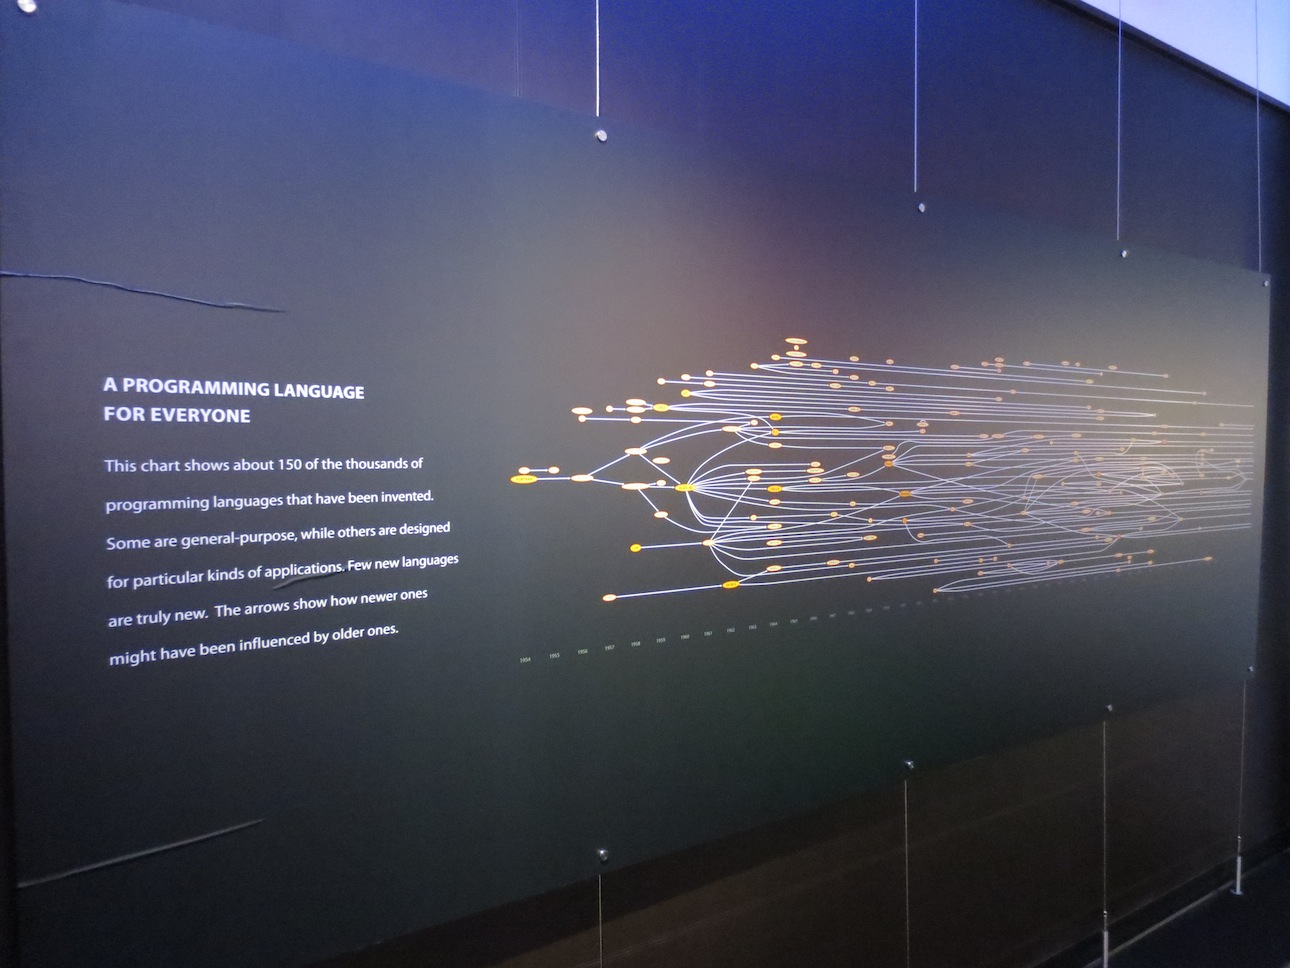
\includegraphics[width=7cm]{programming-languages}
  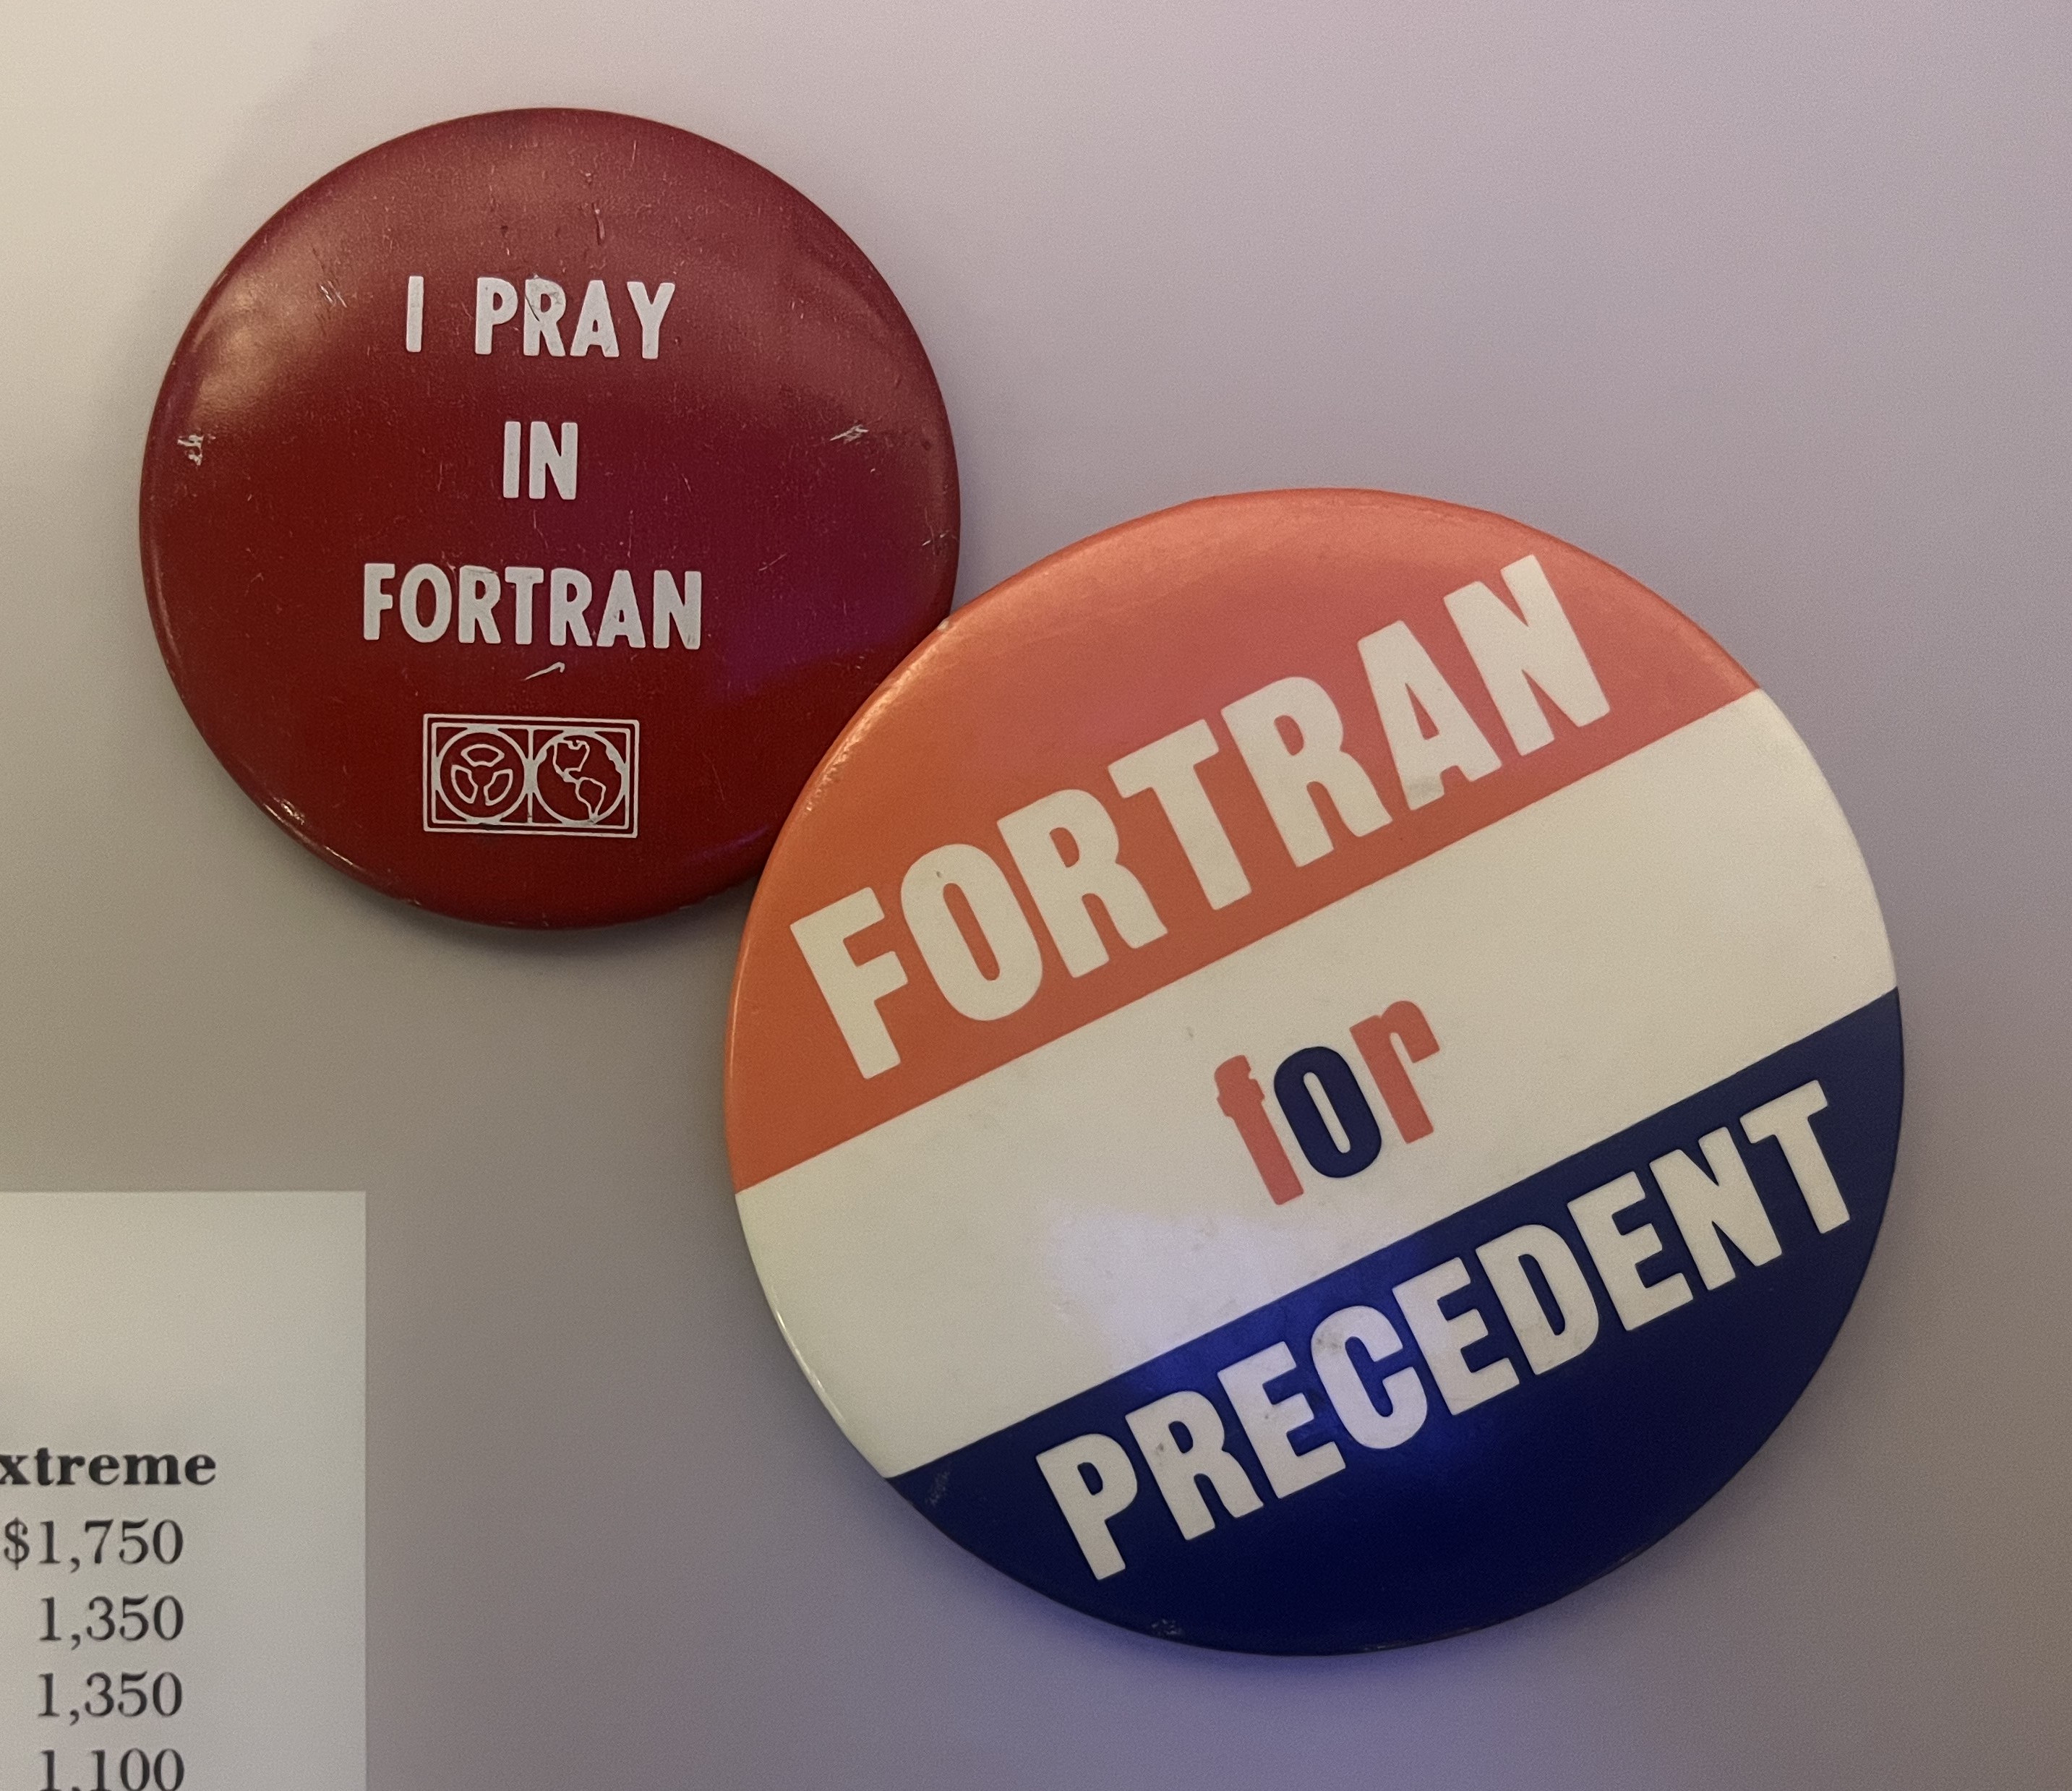
\includegraphics[width=5cm]{fortran-for-precedent}
\end{frame}

\begin{frame}[label=history2]{Don't worry, we are still programming in Fortran, sort of.}
	\centering
	\includesvg[scale=0.85, pretex=\tiny]{languages}

	{\footnotesize ``John [Backus] was very impressed... he always knew that... he needed to figure out how to work mutation into functional programming
	and... generic programming is functional programming with a well-defined way to handle mutation.''
	(Sean Parent, 2018, \emph{`Greatest Common Measure'}, \href{https://youtu.be/FtZEU9zv9eM}{\texttt{youtu.be/FtZEU9zv9eM}})}
\end{frame}

\begin{frame}[label=fortran-comparison,fragile]{2D arrays: Fortran 90 vs \textsc{Multi}}
\small
\begin{tabular}{@{}lll@{}}
\hline
\textbf{Operation}         & \textbf{Fortran 90}                  & \textbf{C++ Multi} \\
\hline
Declaration (3$\times$3)   & \lstinline|real(8) :: A(3,3)|        & \lstinline|multi::array<double,2> A({3,3});| \\
Allocatable                & \lstinline|real(8), allocatable :: A(:,:)| & \lstinline|multi::array<double,2> A;| \\
Allocation                 & \lstinline|allocate(A(10,5))|        & \lstinline|A.reextent({10,5});| \\
Element access             & \lstinline|A(i,j)|                   & \lstinline|A[i][j]| or \lstinline|A(i,j)| (zero-index)\\
First row                  & \lstinline|A(1,:)|                   & \lstinline|A[0]| or \lstinline|A(0,_)| \\
First column               & \lstinline|A(:,1)|                   & \lstinline|A(_,0)| \\
Subblock                   & \lstinline|A(1:2, 1:2)|              & \lstinline|A({0,2},{0,2})| \\
Deallocation               & \lstinline|deallocate(A)|            & \lstinline|A.clear()| \\
\hline
\end{tabular}

\vspace{0.5em}
\begin{alertblock}{Key differences}
  Fortran indices start at \textbf{1}, Multi at \textbf{0}; ranges \lstinline|1:2| are closed, \lstinline|{0,2}| is half-open.
\end{alertblock}
\end{frame}

\begin{frame}[label=numpy-comparison,fragile]{2D arrays: NumPy (Python) vs \textsc{Multi} (C++)}
\small
\begin{tabular}{@{}lll@{}}
\hline
\textbf{Operation}         & \textbf{NumPy}                           & \textbf{C++ Multi} \\
\hline
Uninitialized (3$\times$3) & \lstinline|A = np.empty((3,3))|          & \lstinline|multi::array<double,2> A({3,3});| \\
Zero-filled (3$\times$3)   & \lstinline|A = np.zeros((3,3))|          & \lstinline|multi::array<double,2> A({3,3}, 0.0);| \\
Element access             & \lstinline|A[i,j]|                       & \lstinline|A[i][j]| or \lstinline|A(i,j)| (or in C++23 \lstinline|A[i,j]|) \\
First row                  & \lstinline|A[0]| or \lstinline|A[0,:]|   & \lstinline|A[0]| \\
First column               & \lstinline|A[:,0]|                       & \lstinline|A(_,0)| \\
Subblock                   & \lstinline|A[0:2, 0:2]|                  & \lstinline|A({0,2},{0,2})| \\
Strided slice              & \lstinline|A[::2, :]|                    & \lstinline|A.strided(2)| \\
Shape / extent             & \lstinline|A.shape|                      & \lstinline|A.extensions()| \\
View (zero-copy)           & \lstinline|B = A[0:2]| (view)            & \lstinline|auto&& B =  A({0,2});| (subarray) \\
Copy                       & \lstinline|B = A[0:2].copy()|            & \lstinline|auto   B =+ A({0,2});| \\
GPU array                  & \lstinline|cupy.array(...)|              & \lstinline|multi::thrust::array<double,2>| (type alias) \\
\hline
\end{tabular}

\vspace{0.4em}
\begin{alertblock}{Key differences}
  NumPy slices use \textbf{closed-open} \lstinline|[0:2]| ranges --- same as Multi \lstinline|{0,2}|.
  Multi subarrays are \textbf{always views}; a copy requires an explicit syntax.
  Multi's type encodes rank and element type at compile time $\Rightarrow$ zero overhead, GPU portability.
\end{alertblock}
\end{frame}

\begin{frame}[label=history3]{We need philosophy (mathematics) to program, especially libraries}
	\begin{quote}
		What kind of programs are not mathematical? Programs that are insecure, programs that
		crash, programs that cannot be easily modified are examples of non-mathematical software.
		There is, of course, a solid economic reason for producing such programs: they assure
		world domination on a large scale and job security on a small scale. -- Alex Stepanov, \emph{Notes on the foundations of programming, 2005}
	\end{quote}

	\noindent\makebox[\linewidth]{\resizebox{0.3333\linewidth}{1pt}{$\bullet$}}\pause

	\begin{quote}
		[Guys!] We should use formal methods even when we write XML stuff. -- Alex Stepanov (2003), \href{https://youtu.be/fanm5y00joc?t=6723}{\texttt{youtu.be/fanm5y00joc}}
	\end{quote}
\end{frame}

\begin{frame}[label=motivation1]{Why Multidimensional Arrays?}
  \begin{columns}
    \begin{column}{0.5\textwidth}
      \textbf{Scientific computing is array computing}
      \begin{itemize}
        \item Discretized PDEs: 2D/3D grids
        \item Quantum chemistry: matrices, tensors
        \item Signal processing: time $\times$ frequency
        \item Machine learning: batches $\times$ features $\times$ channels
      \end{itemize}
      \pause
      \vspace{0.8em}
      \textbf{Performance lives in arrays}
      \begin{itemize}
        \item Contiguous/Regular memory $\Rightarrow$ cache efficiency
        \item SIMD vectorization, GPU parallelism
        \item BLAS/LAPACK/FFTW operate on array layouts
      \end{itemize}
      \pause
    \end{column}
    \begin{column}{0.5\textwidth}
      \textbf{Arrays are a natural abstraction}
      \begin{itemize}
        \item Most algorithms iterate over index ranges
        \item Lingua franca: Fortran, APL, Matlab, NumPy built around them
        \item C++ STL: ranges of elements --- but only 1D
      \end{itemize}
      \vspace{0.8em}
      \begin{alertblock}{The gap (A blessing in disguise)}
        C++ has no standard multidimensional array with
        value semantics, subarrays, and algorithm support.
      \end{alertblock}
    \end{column}
  \end{columns}
\end{frame}

\begin{frame}[plain,label=motivation2]{Motivating example: Electron density \(\rho\) reacts to swift atomic motion}
\begin{columns}
  \begin{column}{0.4\textwidth}
    \includesvg[width=\textwidth]{electron_density}
  \end{column}
  \begin{column}{0.6\textwidth}
     \movie[width=1.05\textwidth, height=0.8055\textwidth, autostart, loop]{%
    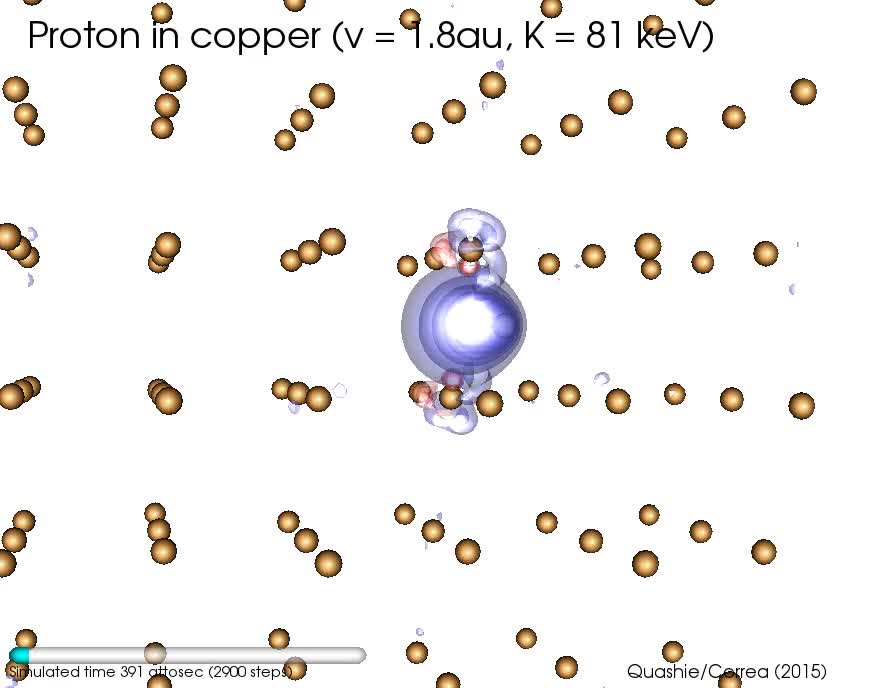
\includegraphics[width=1.05\textwidth]{diff-movie_v1p8au_contour}%
  }{diff-movie_v1p8au_contour.mp4}
  \end{column}
\end{columns}
\end{frame}

{
  \usebackgroundtemplate{
    %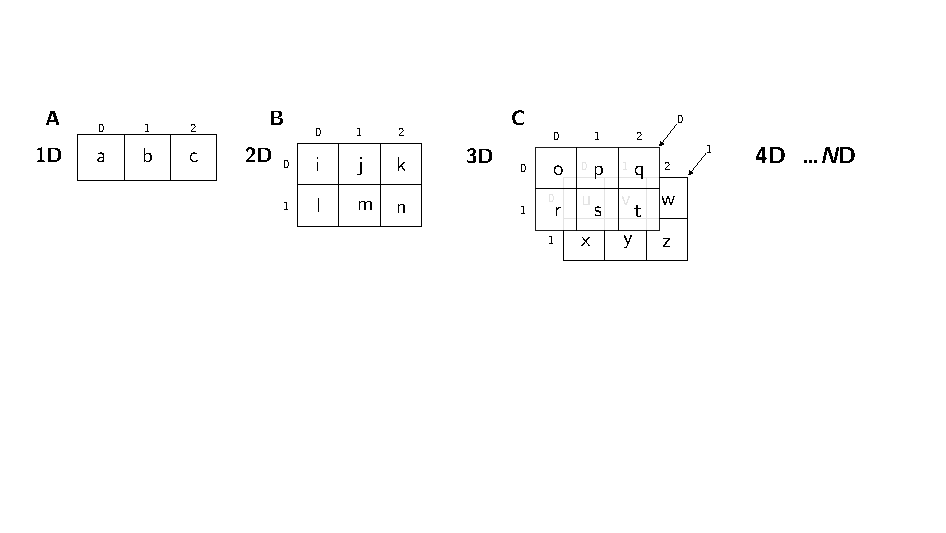
\includegraphics{arrays_1D_2D_3D_4D_ND}
    \includesvg[width=\paperwidth,inkscapelatex=false]{arrays_1D_2D_3D_4D_ND}
  }
\begin{frame}[label=intro1,fragile]{What are multidimensional Arrays}
\vspace{3cm}
\begin{lstlisting}
  assert( A[1] == 'b' );         // A(1)
  assert( B[1][2] == 'n' );      // B(1, 2)
  assert( C[1][0][2] == 'w' );   // C(1, 0, 2)
\end{lstlisting}
\begin{alertblock}{Visualization is only a convention}
  Implies a symmetry in the indices.
\end{alertblock}
\end{frame}

\begin{frame}[fragile]{Multidimensional Arrays}
\vspace{3cm}
\begin{lstlisting}
  assert( A != B[0] );
  assert( C(0, {0, 2}, {0, 2}) != B );
\end{lstlisting}
\begin{alertblock}{Expected behavior across dimensions}
  There are relations across dimensions
\end{alertblock}
note: most examples in this talk are 2D for simplicity, imagine the ND generalization
\end{frame}
}

\begin{frame}
\frametitle{C++ and multidimensional arrays in 2026\ldots}

\begin{block}{Keynote: ``Making C++ Standard Parallelism Multidimensional''}
  \begin{itemize}
    \item Do not miss this keynote by Mark Hoemmen (NVIDIA)
  \end{itemize}
\end{block}
\begin{itemize}
  \item `Typed linear algebra' by François Carouge
  \item \textsc{Parrot} library by Conor Hoekstra (NVIDIA) \href{https://github.com/NVlabs/parrot}{\texttt{github.com/NVlabs/parrot}}
  \item CUDA Tile soon to be available for C++
  \item \textsc{Boost.Multi} (this work) fully accepted? \emoji{crossed-fingers}
\end{itemize}

\bigskip
\begin{alertblock}{2026}
  \large Is 2026 \textbf{the year of C++ as an array language}? \emoji{smiley}
\end{alertblock}

\end{frame}

\begin{frame}[label=strided1]{Strided arrays as a data structure, subarray subblock}
\vspace{-1.4cm}
\includesvg[width=\paperwidth]{strided_subblock}

\url{https://godbolt.org/z/1M3Eb3fhj}
\end{frame}

\begin{frame}[label=strided2]{Strided arrays as a data structure, row subarray}
\vspace{-1.4cm}
\includesvg[width=\paperwidth]{strided_row}

\url{https://godbolt.org/z/1M3Eb3fhj}
\end{frame}

\begin{frame}[label=strided3]{Strided arrays as a data structure, column subarray}
\vspace{-1.4cm}
\includesvg[width=\paperwidth]{strided_col}

\url{https://godbolt.org/z/1M3Eb3fhj}
\end{frame}

\begin{frame}[label=strided4]{Strided arrays as a data structure, strided subarray}
\vspace{-1.4cm}
\includesvg[width=\paperwidth]{strided_subblock_stride}

\url{https://godbolt.org/z/1M3Eb3fhj}
\end{frame}

\begin{frame}[label=strided5]{Strided arrays as a data structure}
\begin{center}
\lstinline|element i, j ->   base + stride1*i + stride2*j|
\end{center}

Pros:
\begin{itemize}
  \item Maintains symmetry as much as possible between dimensions
  \item Memory of arrays and subarrays is compact, regular, and often contiguous
  \item Compatible with legacy libraries, FFTW, BLAS, LAPACK, cuFFT, cuBLAS, MPI
\end{itemize}
Cons:
\begin{itemize}
  \item Not available in the language; needs library solutions
  \item No support from STL algorithms
  \item Not easy to grow
\end{itemize}

\begin{alertblock}{Other data structures (layouts) also maintain symmetry}
  Tiled, Zig-zag, Hilbert curve filling
\end{alertblock}

\end{frame}

\begin{frame}{Multidimensionality via nested containers (the wrong way)}
\begin{columns}[T]
\begin{column}{0.5\textwidth}
\lstinline|std::vector<std::vector<T> >|

\includesvg[scale=0.8]{nested_vector}
\end{column}
\begin{column}{0.5\textwidth}
Pros (mostly traps)
\begin{itemize}
  \item \texttt{B[i][j]} works out of the box
  \item Iterator access available (but only if you access things the right way)
  \item Easy to grow (in the first dimension)
\end{itemize}
Cons:
\begin{itemize}
  \item Distinct logic for different dimensions
  \item Memory all over the place
  \item Has to maintain invariant (rectangular size)
  \item Not compatible with legacy libraries
  \item Gets worse with higher dimensionality
\end{itemize}
\end{column}
\end{columns}
\end{frame}

\section{Generic Programming Foundations}

\begin{frame}[fragile]{Semiregular types (Stepanov Regularity, EoP)}
	\begin{center}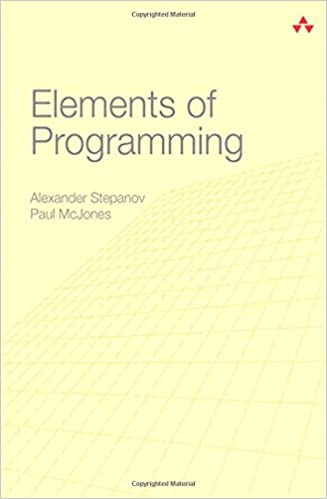
\includegraphics[height=3cm]{eop}\end{center}
	\begin{lstlisting}
struct SR {
	 SR();  // default constructible
	 SR(SR const& other);  // copy constructible
	~SR();  // destructible
	auto operator=(SR const& r) -> R&;  // assignment
};
\end{lstlisting}
  ... and also the semantics should be as expected

	Available algorithms: \emph{swap} (\lstinline{std::swap})
\end{frame}

\begin{frame}[fragile]{Regular = Semiregular + has equality}

	\begin{lstlisting}
struct R { ...
	auto operator==(R const& other) const -> bool;
	auto operator!=(R const& other) const -> bool;  // neg
};
\end{lstlisting}
	\pause
	in C++20
	\begin{lstlisting}
struct R { ...
	auto operator==(R const& other) const -> bool;  // = default;
	// ^^^ synthesizes !=
};
\end{lstlisting}

Some types might not have equality in practice because equality could be prohibitively expensive or the algorithm for equality is not known.

Available algorithms: \emph{linear-search} (\lstinline{std::find})
\end{frame}

\begin{frame}[fragile]{PartialOrder = Regular + has order}

	\begin{lstlisting}
struct PO { ...
	bool operator< (PO const& other) const;
	bool operator> (PO const& other) const;
	bool operator>=(PO const& other) const;
	bool operator<=(PO const& other) const;
};
\end{lstlisting}
	\pause
	in C++20
	\begin{lstlisting}
struct PO { ...
	auto operator== (P const& other) const = default;
	auto operator<  (P const& other) const = default;
	auto operator<=>(P const& other) const = default;
	// ^^^ synthesizes <=, >=, >,
};
\end{lstlisting}

	Available algorithms: \emph{sort} (\lstinline{std::sort}), \emph{binary-search} (\lstinline{std::lower_bound})
\end{frame}

\begin{frame}[fragile]{TotalOrder = PartialOrder + has trichotomy}

trichotomy: Not $a < b$ and not $a > b$ $\Rightarrow a == b$

\begin{lstlisting}
struct TO { ...
	bool operator< (TO const& other) const;
	bool operator> (TO const& other) const;
	bool operator>=(TO const& other) const;
	bool operator<=(TO const& other) const;
};
\end{lstlisting}

	in C++20
	\begin{lstlisting}
struct TO { ...
	auto operator<  (TO const& other) const = default;
	auto operator<=>(TO const& other) const = default;
	// ^^^ synthesizes ==, !=, >, <=, >=
};
\end{lstlisting}

Available algorithms: same as before, but they can be more efficient.

\end{frame}

\begin{frame}[fragile]{Claim: (Semi)Regular types are amenable to equational reasoning.}

	\underline{Modern C++ is based around them}

	\begin{alertblock}{Litmus test for your specific type \lstinline{Type}}
		Quick test for your types, does this compile? Does it do the expected thing?
\begin{lstlisting}
std::vector<Type> v = {r1, r2, r3};
std::sort( v.begin(), v.end() );
assert( std::is_sorted(v.begin(), v.end() ) );
\end{lstlisting}
\end{alertblock}

A number of classes in libraries (or frameworks) do \textbf{not} pass the litmus test.
\begin{lstlisting}
coocooLib_array a; coocooLib_array b;
a = b;  // look how smart (?), a now "points" to b
a.copy(b);  // inflation of syntax
a.deep_copy(); a.really_copy(b); a.NoJoke_copy(b);
\end{lstlisting}

\end{frame}

\begin{frame}[fragile]{Values = Regular + platonic / persistent}

Values are Regular types that are also amenable to \emph{mathematical}, \emph{equational}, \emph{logical} reasoning, e.g. \emph{arithmetic}.
Mathematics and numerical mathematics are based around them.

\pause

Values = Regular + saving/loading to a medium (serialization)

\begin{lstlisting}
struct Value { ...
	void save(Archive& ar) const;
	void load(Archive& ar);
};
\end{lstlisting}
	\begin{lstlisting}
void print(Value const&); void read(Value &);
\end{lstlisting}
	\begin{lstlisting}
auto operator<<(std::ostream& out, Value const& self) {...}
auto operator>>(std::istream& out, Value &      self) {...}
\end{lstlisting}

	\begin{alertblock}{Drawback}
		There is no standard way to serialize in C++.
		It is up to us to adopt a convention, protocol(s) or a standard.
	\end{alertblock}

	Boost.Serialization, Cereal, Google's protobuf, ...
\end{frame}

\section{Array Model}

\begin{frame}[label=boost1]{\textsc{Multi} was proposed to Boost (2026) and conditionally accepted}
\begin{columns}
\begin{column}{0.6\textwidth}
\href{https://gitlab.com/correaa/boost-multi}{\texttt{gitlab.com/correaa/boost-multi}}\\
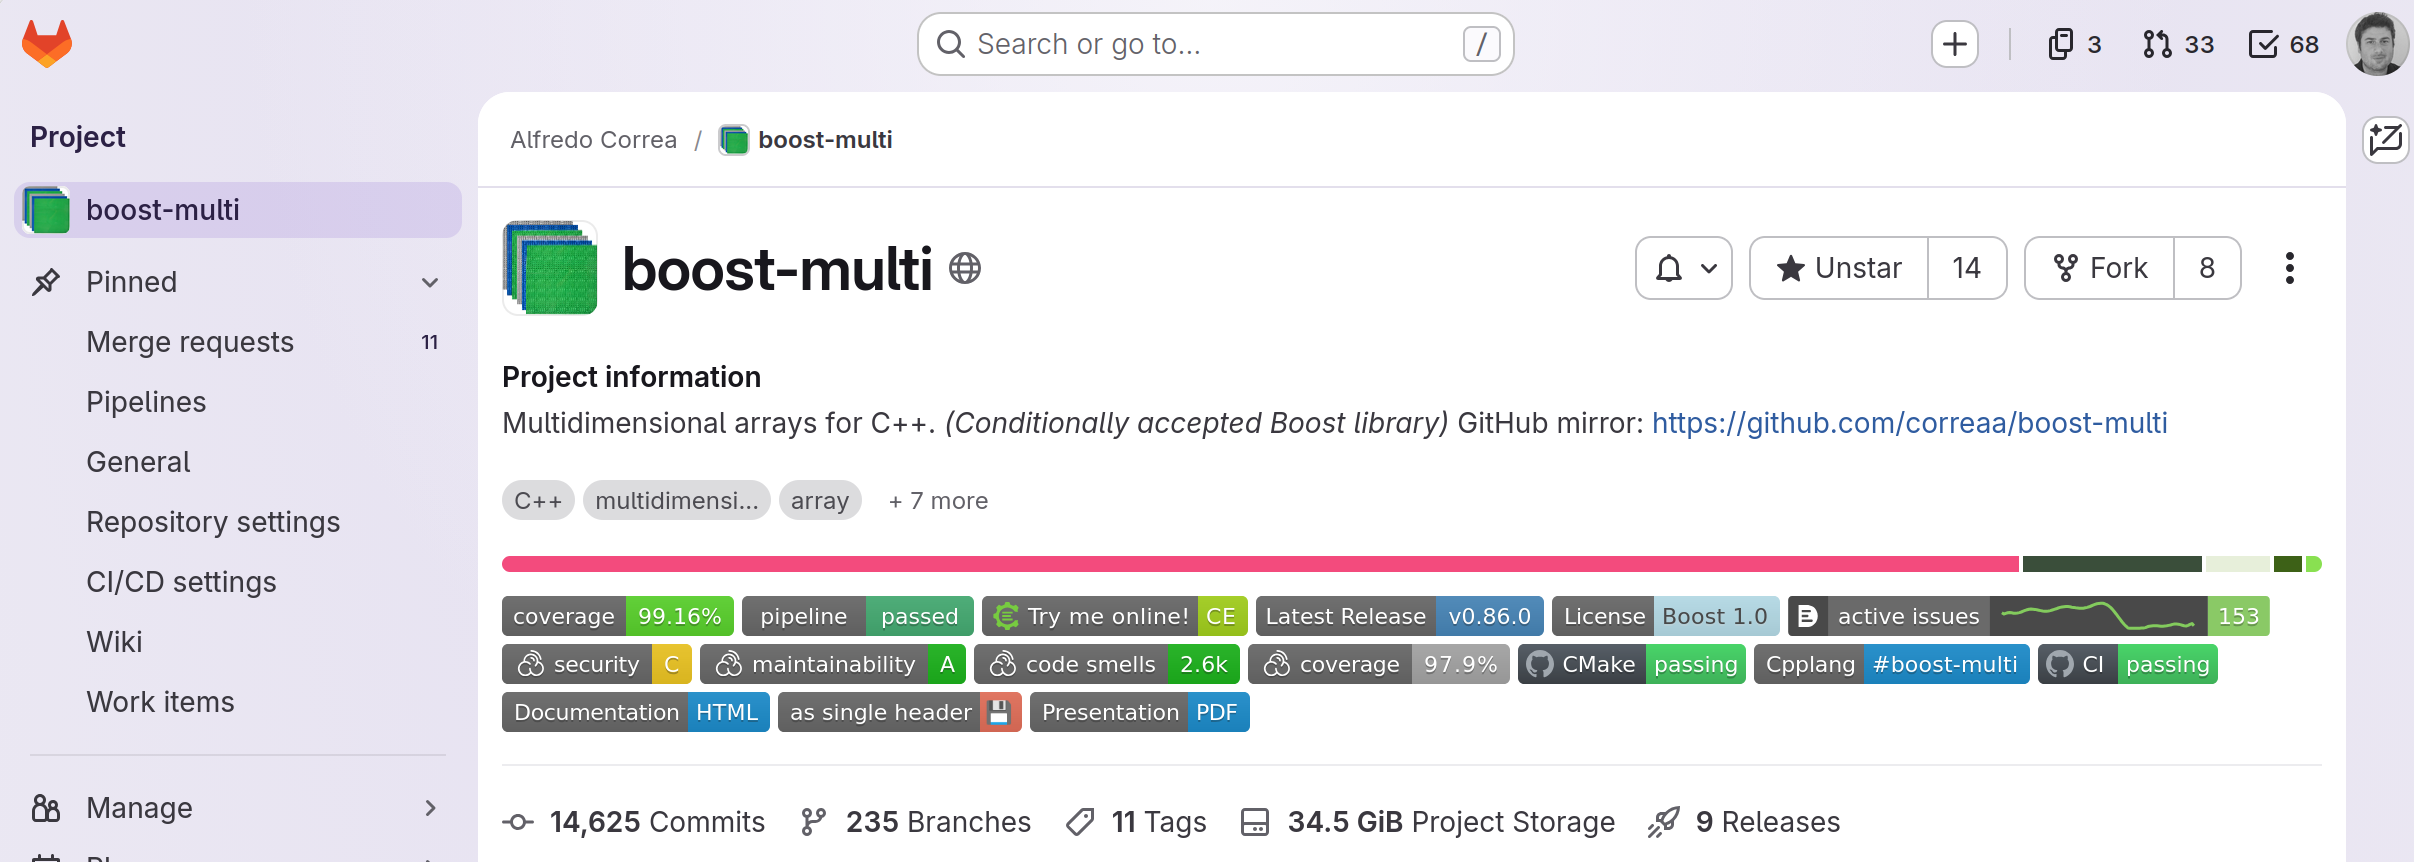
\includegraphics[scale=0.1]{gitlab}\\
\href{https://github.com/correaa/boost-multi}{\texttt{github.com/correaa/boost-multi}}\\
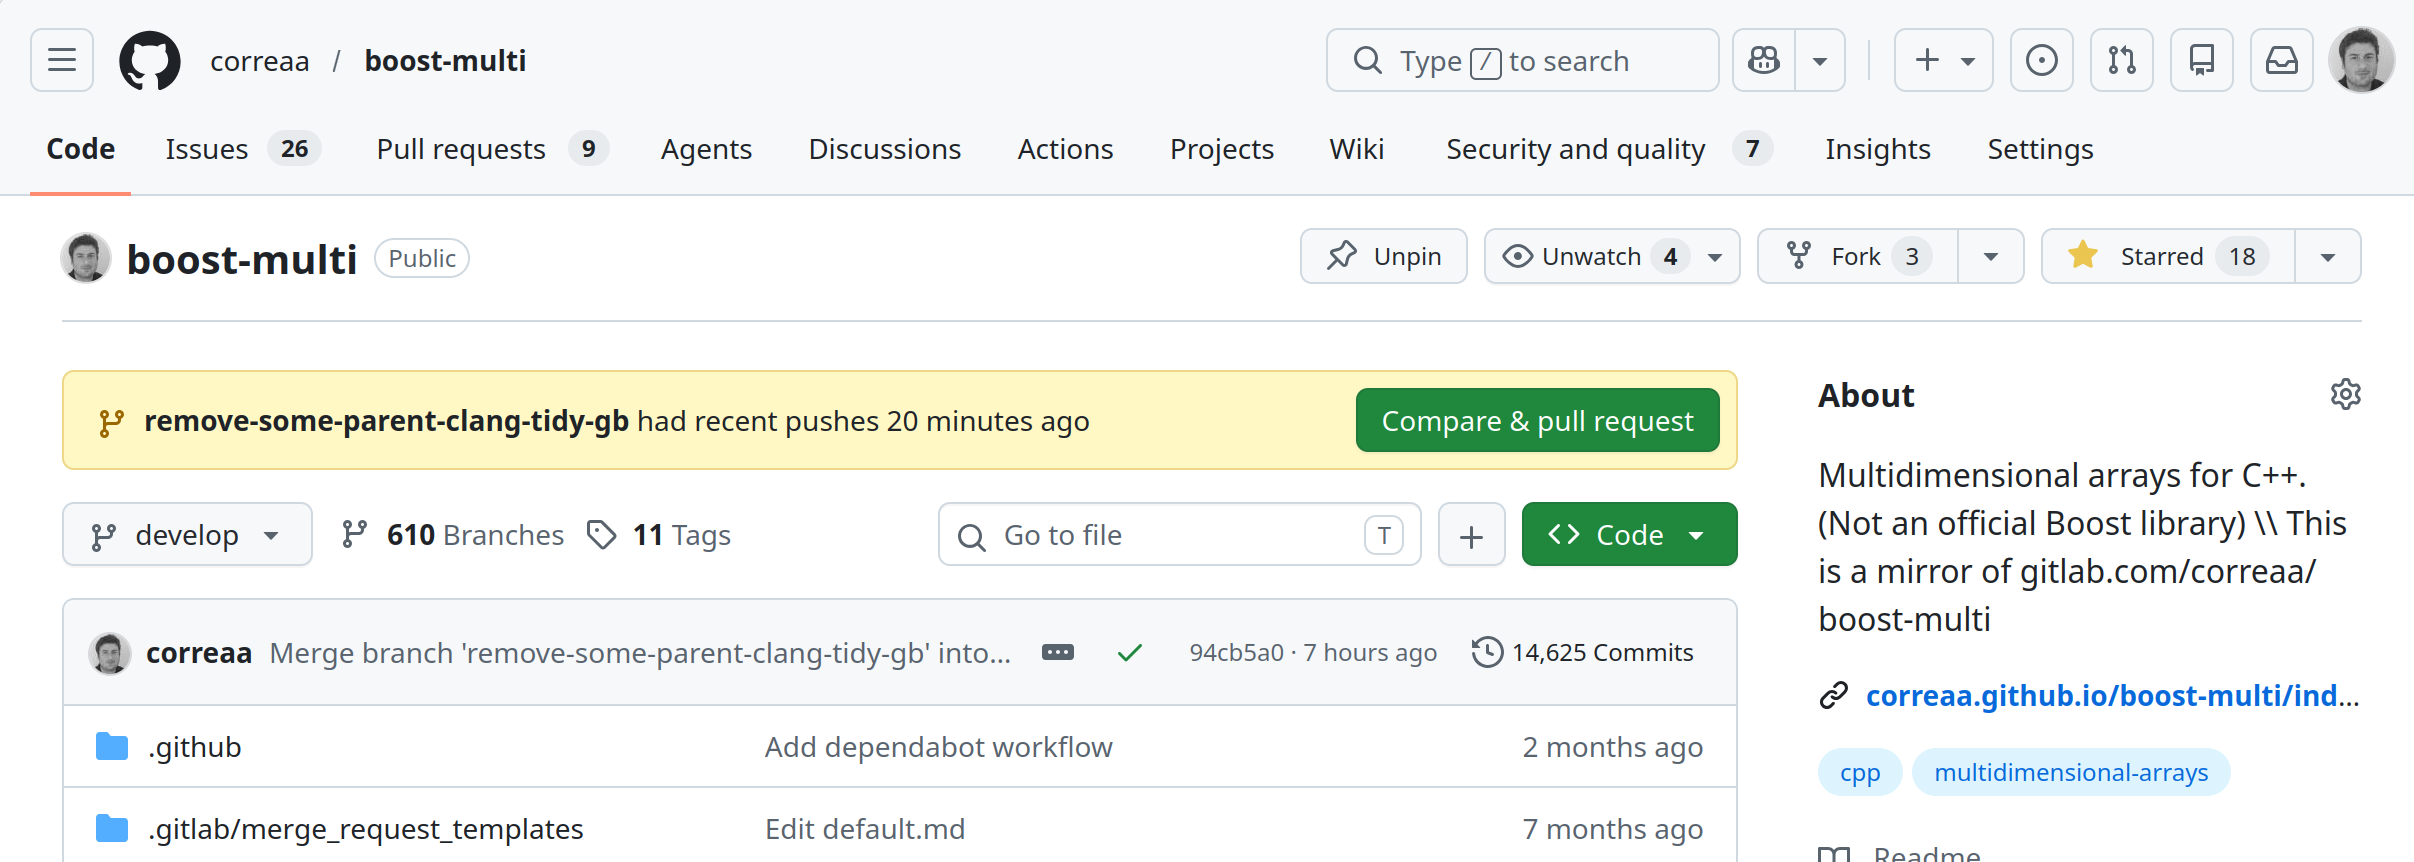
\includegraphics[scale=0.1]{github}\\
\end{column}
\begin{column}{0.4\textwidth}
\href{https://correaa.github.io/boost-multi}{\texttt{correaa.github.io/boost-multi}}\\
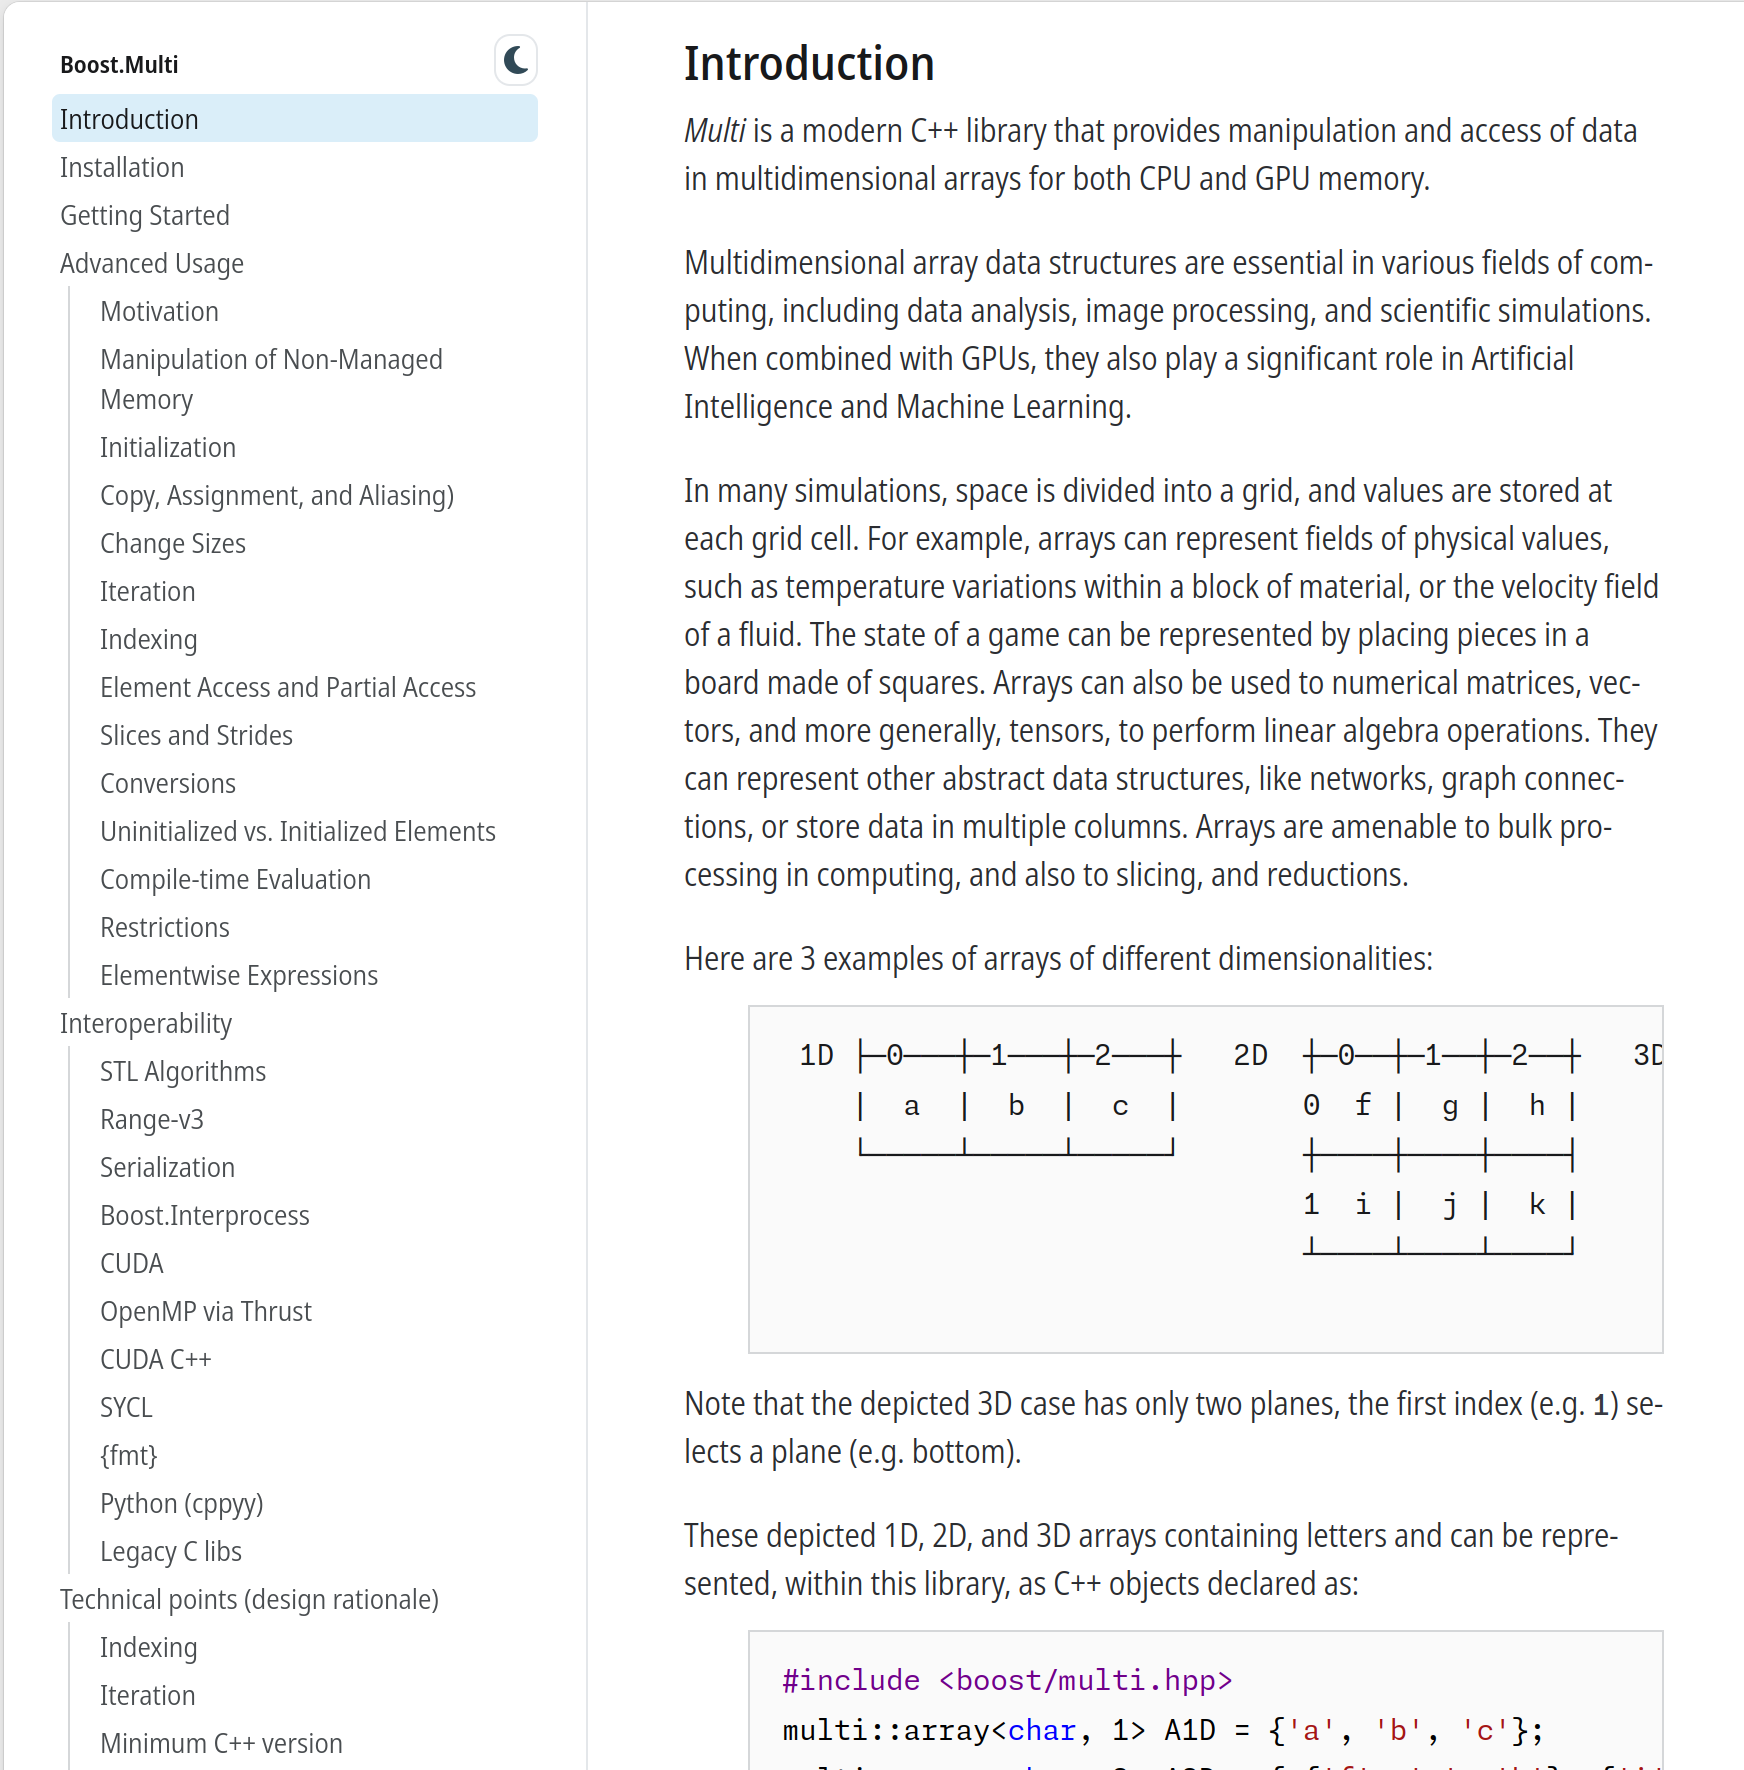
\includegraphics[scale=0.1]{documentation}\\
\footnotesize{Thanks Matt Borland @ CPPAlliance!}
\end{column}
\end{columns}

\end{frame}

\begin{frame}[label=boost2]
\frametitle{\textsc{Multi} proposed to Boost}
Why \textbf{not} proposed for Standard (or Beaman)?
\begin{itemize}
  \item Can't promise (ABI) compatibility
  \item Controversial idioms (some hacks) \emoji{hot-pepper}
  \item Too restrictive for compatibility with exotic 3rd parties (Thrust, BLAS, CUDA, cuLibs)
  \item Enough overlap with \texttt{std::span}, \texttt{std::mdspan} and \texttt{std::mdarray}
  \item Long time horizon (I am stuck in C++17/20 for compatibility with GPUs)
\end{itemize}

Why proposed to Boost?
\begin{itemize}
  \item Ideal balance between risk (innovation) and requirements (quality, guidelines)
  \item \emph{Peer reviewed}
  \item Still good distribution model and visibility
  \item No need for compiler-magic
  \item Moderate time horizon
  \item Can eventually benefit from low-level Boost tools (Boost.Hana, Boost.Assert, Boost.Align, Boost.STLInterfaces)
  \item Peer interaction with Boost.Serialization, Boost.JSON, Boost.QVM, Boost.YAP
\end{itemize}
\end{frame}

\begin{frame}[label=uses1]{Real world uses}
  \begin{itemize}
    \item INQ: engine for electronic structure calculations and dynamics, LLNL
    \item QMCPACK: Quantum Monte Carlo (QMC) simulation code, Oak Ridge Natl Lab
    \item CoQuí: Correlated Quantum Systems (post-DFT: GW, RPA, THC-AFQMC) Flatiron Institute, NY
    \item Dalotia: data loader library for tensors in AI, RIKEN (RCCS), Japan
  \end{itemize}
\end{frame}

\begin{frame}[label=uses2]{Abinitio C++ Codes INQ (DFT/TDDFT) \& QMCPACK (QMC/AFQMC)}
	\centering
	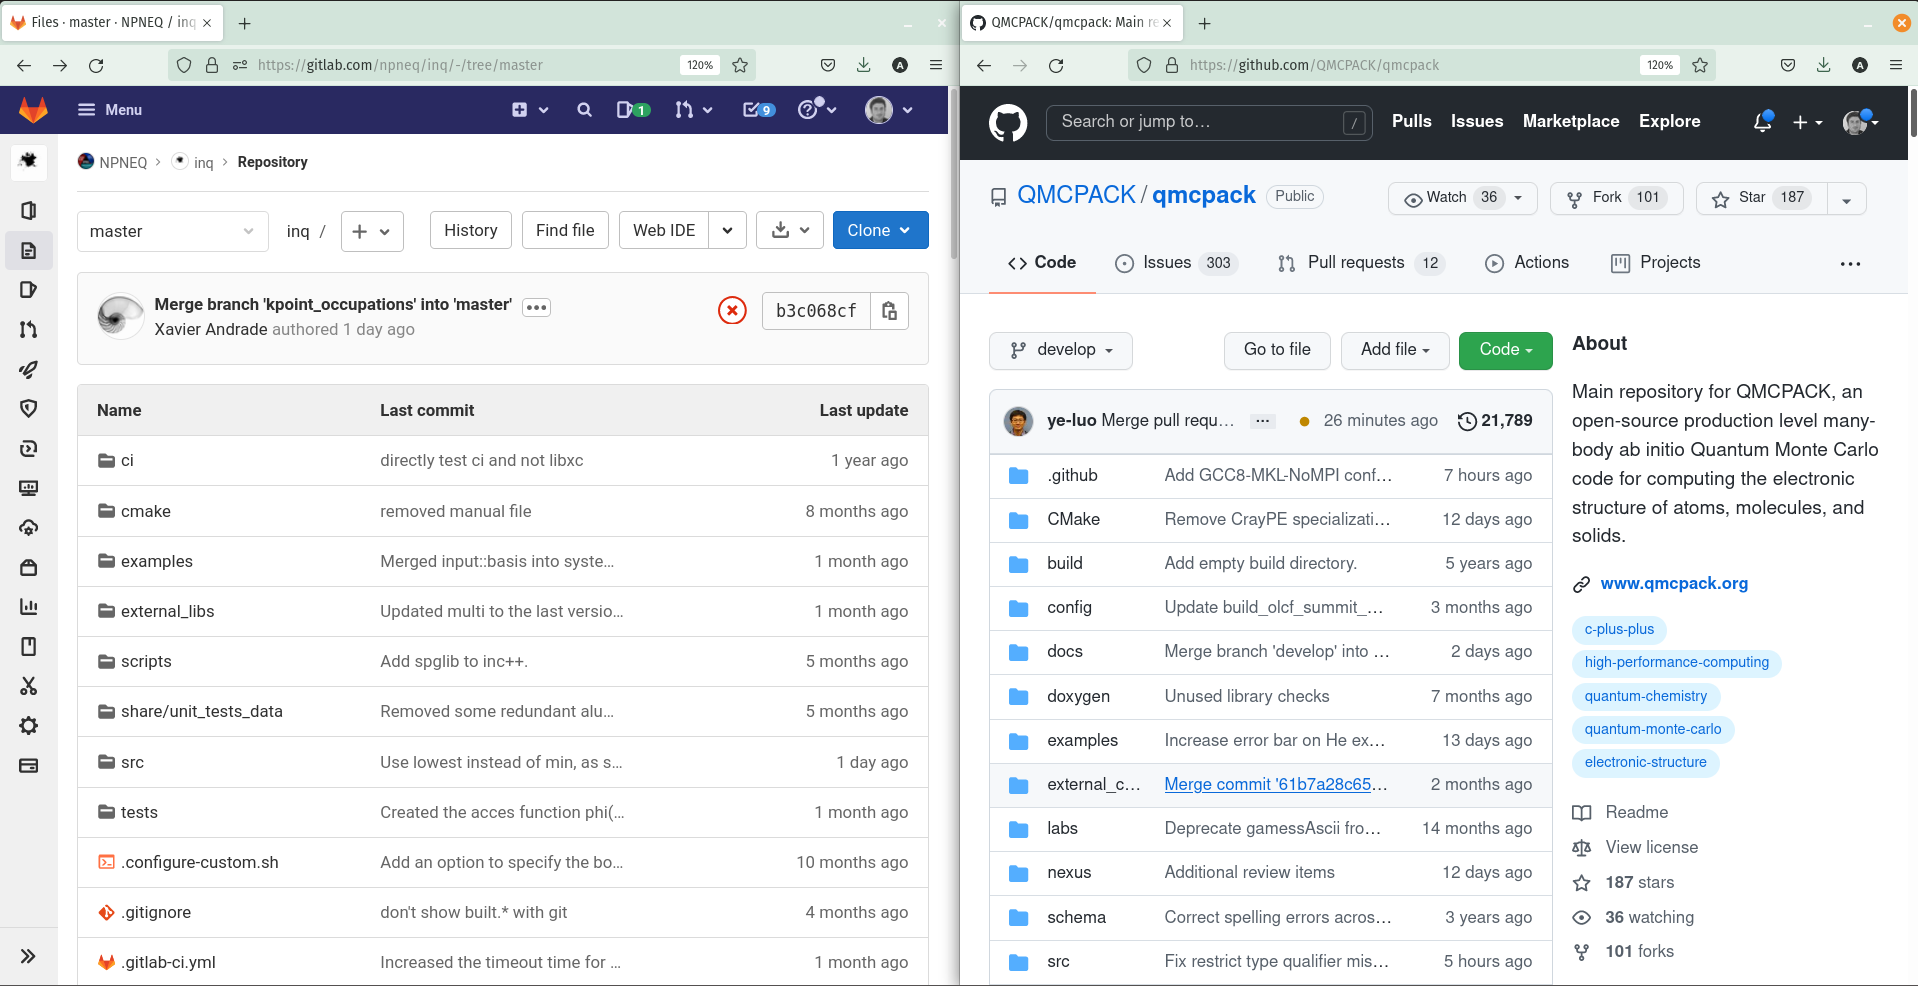
\includegraphics[width=0.75\columnwidth]{git_screenshots}
	\begin{alertblock}{Observation}
		C++ has become the \emph{de facto} standard for HPC. We better create a good ecosystem.
	\end{alertblock}
\end{frame}

\begin{frame}[label=inq1]{INQ, electronic structure code for HPC systems}
	\centering
	\includesvg{dependencies}

  Individual components can be shared and reused by other projects
\end{frame}

\begin{frame}[fragile,label=basic1]{Construction and basic usage}
\begin{lstlisting}
#include <boost/multi/array.hpp>
namespace multi = boost::multi;
// from extents
multi::array<int, 2> A({3, 4});  // a 3 x 4 array

// from a (rectangular) initializer list
multi::array<int, 2> B = {{1, 2, 3}, {4, 5, 6}};

// from existing memory (no allocation, no ownership)
int data[12] = {};
multi::array_ref<int, 2> C({3, 4}, data);

// element access
A(1, 2) = 5;  // equivalent
A[1, 2] = 5;  // equivalent C++23
A[1][2] = 5;  // intermediate object?
\end{lstlisting}
\end{frame}

\begin{frame}[fragile,label=basic2]{Proxy subarray-reference}
\begin{center}
\includesvg[scale=0.7]{strided_row_small}
\end{center}
\begin{lstlisting}
multi::array<int, 2> A({4, 6});
??? row = A[1];  // same as A(1, _) or *(A.begin() + 1)
// choose one:
auto                       row = ...  // misleading, valid but not recommended
multi::subarray<double, 1> row = ...  // too verbose, but correct
multi::array<double, 1>    row = ...  // correct, but makes a copy
auto&&                     row = ...  // self-documenting
\end{lstlisting}

\begin{alertblock}{The problem with \texttt{auto}: ``Implicit Evaluation of `auto' Variables.''}
P0672R0 (2017) by Jo\"el Falcou, Herb Sutter et al.
(\texttt{std::vector<bool>}, proxy objects)
\end{alertblock}

\end{frame}

\begin{frame}[fragile,label=basic3]{My recommendation (unenforceable, opt-in)}
\begin{itemize}
  \item Use the provided `auto-plus' operator
  \item Rely on lifetime extensions \emoji{hot-pepper} to document naming of reference-subarrays
\end{itemize}
\begin{lstlisting}
multi::array<double, 2> A({3, 4});

auto        row = + A[1];  // multi::array<double, 1>          row = A[1];
auto&&      row =   A[1];  // multi::subarray<double, 1>       row = A[1];
auto const& row =   A[1];  // multi::const_subarray<double, 1> row = A[1];
\end{lstlisting}

Prefer forward (universal) references:
\begin{lstlisting}
template<class Array2D>
  // constrains, e.g. dimensionality == 2
auto f(Array2D&& arr) { ... }
\end{lstlisting}

Want to avoid bloat? (or work across compilation boundaries?)
\begin{lstlisting}
auto g(multi::subarray<int, 2> arr) { ... }
\end{lstlisting}
\end{frame}

\begin{frame}[fragile,label=basic4]{Fundamental access/layout operations}
Indexing
\begin{itemize}
\item Index\\
  \lstinline|A[i]| removes (binds) first dimension
\item Slice\\
  \lstinline|A.sliced(first, last)| range subarrays (equal dimension) half-open interval \([\mathrm{first}, \mathrm{last}) \)
\end{itemize}

Fundamental
\begin{itemize}
\item Rotate (indices) \\
  \lstinline|A.rotated()[i][j][k] == A[k][i][j]|
\item Unrotate (indices) \\
  \lstinline|A.unrotated()[i][j][k] == A[j][k][i]|
\item Transpose (first two indices) \\
  \lstinline|A.transposed()[i][j][k] == A[j][i][k]|
\item Strided
  \lstinline|A.strided(n)[i] == A[n*i]|
\end{itemize}
\end{frame}

\begin{frame}[fragile,label=basic5]{Derived and positional indexing}
\begin{itemize}
  \item Indexing (with parentheses)
    \lstinline|A(i) -> A[i]|
  \item Sliced (terse)
    \lstinline|A({first, last}) -> A.sliced(first, last)|
  \item Generalized slice:\\
    \lstinline|A({first, last, every}) -> A.sliced(first, last).strided(every)|
  \item Row\\
    \lstinline|A(i, _) -> A[i](_) -> A[i]| \\
  \item Column\\
    \lstinline|A(_, i) -> A.rotated()[i]| \\
  \item Partial column\\
    \lstinline|A({first, last}, i) -> A.rotated()[i]({first, last})| \\
\end{itemize}

\begin{block}{Too many temporaries objects?}
Modern compilers can elide these temporary objects.
\end{block}

\begin{alertblock}{}
  Since C++23 you can use multidimensional square brackets \lstinline|A[i, j, k]|
\end{alertblock}
\end{frame}

\begin{frame}[fragile]{Aliasing and how to break it}
\begin{lstlisting}
  multi::array<int, 2> A({3, 3});
  multi::array<int, 2> B({3, 3});
  multi::array<int, 2> C;

  B = A.transposed();  // ok  allocates?
  C = A.transposed();  // ok  allocates?

  A = A.transposed();  // ok? aliasing!

  A = + A.transposed();  // ok allocates?
\end{lstlisting}

\begin{alertblock}{Dual purpose of operator+}
  \begin{itemize}
    \item Help \texttt{auto}
    \item Materialize [sub]array-references
  \end{itemize}
\end{alertblock}
\end{frame}

\begin{frame}[fragile]{Type hierarchy: ownership and mutability}

\begin{table}
\small
\begin{tabular}{cllllll}
\textbf{Type}                              & \textbf{Owns} & \textbf{Copyable}     & \textbf{Move} & \textbf{Swap} & \textbf{Mutable elems?} & \textbf{Resizable} \\
\hline
\lstinline|multi::const_subarray<T, D, P>| & No            & No \emoji{hot-pepper} & No            & No            & No                      & No                 \\
                          ↑                &               &                       &               &               &                         &                    \\
\lstinline|multi::subarray<T, D, P>|       & No            & No \emoji{hot-pepper} & No            & O(N)          & Yes                     & No                 \\
                          ↑                &               &                       &               &               &                         &                    \\
\lstinline|multi::array_ref<T, D, P>|      & No            & No \emoji{hot-pepper} & No            & O(N)          & Yes                     & No                 \\
                          ↑                &               &                       &               &               &                         &                    \\
\lstinline|multi::dynamic_array<T, D, A>|  & Yes           & Yes                   & No            & O(N)          & Yes                     & No                 \\
                          ↑                &               &                       &               &               &                         &                    \\
\lstinline|multi::array<T, D, A>|          & Yes           & Yes                   & Yes           & Yes           & Yes                     & Yes                \\
\end{tabular}
\end{table}

\begin{alertblock}{Inheritance for composition (usually a bad idea)}
  I made it \texttt{public} inheritance \emoji{hot-pepper} because I found it useful.
  It is opt-in.
\end{alertblock}
\end{frame}

\begin{frame}{Relations between types, recursion across dimensions (simplified)}
\centering

\includegraphics[scale=0.75]{types_relations}

\begin{alertblock}{It looks complicated}
Intuitive for the most part in practice. Perhaps arrays deserve this level of complexity.
\end{alertblock}
\end{frame}

\begin{frame}[fragile]{Wait! \texttt{multi::subarray}'s are not copyable? How to "store" subarrays?}
\centering
\includesvg{store_subarrays}

\begin{lstlisting}
std::vector sas = {B({0, 2}, {0, 2}), B({1, 4}, {1, 4}), B({0, 2}, {4, 6})};
// error! subarray<int, 2> is not copyable
\end{lstlisting}

\begin{lstlisting}
std::vector saps = {&B({0, 2}, {0, 2}), &B({1, 4}, {1, 4}), &B({0, 2}, {4, 6})};
// std::vector<multi::subarray_ptr<T, 2>> sarrps = ...
for(auto sap : saps) {
  std::ranges::fill(sap->elements(), 0);
}
\end{lstlisting}
{\raggedleft\href{https://godbolt.org/z/E1EsKn8o5}{\texttt{godbolt.org/z/E1EsKn8o5}}\par}
\end{frame}

\begin{frame}{\textit{``Copy or copy not; there is no shallow. -- Master Yoda''} -- Tony Van Eerd}
\centering
\begin{columns}[T]
\begin{column}{0.5\textwidth}
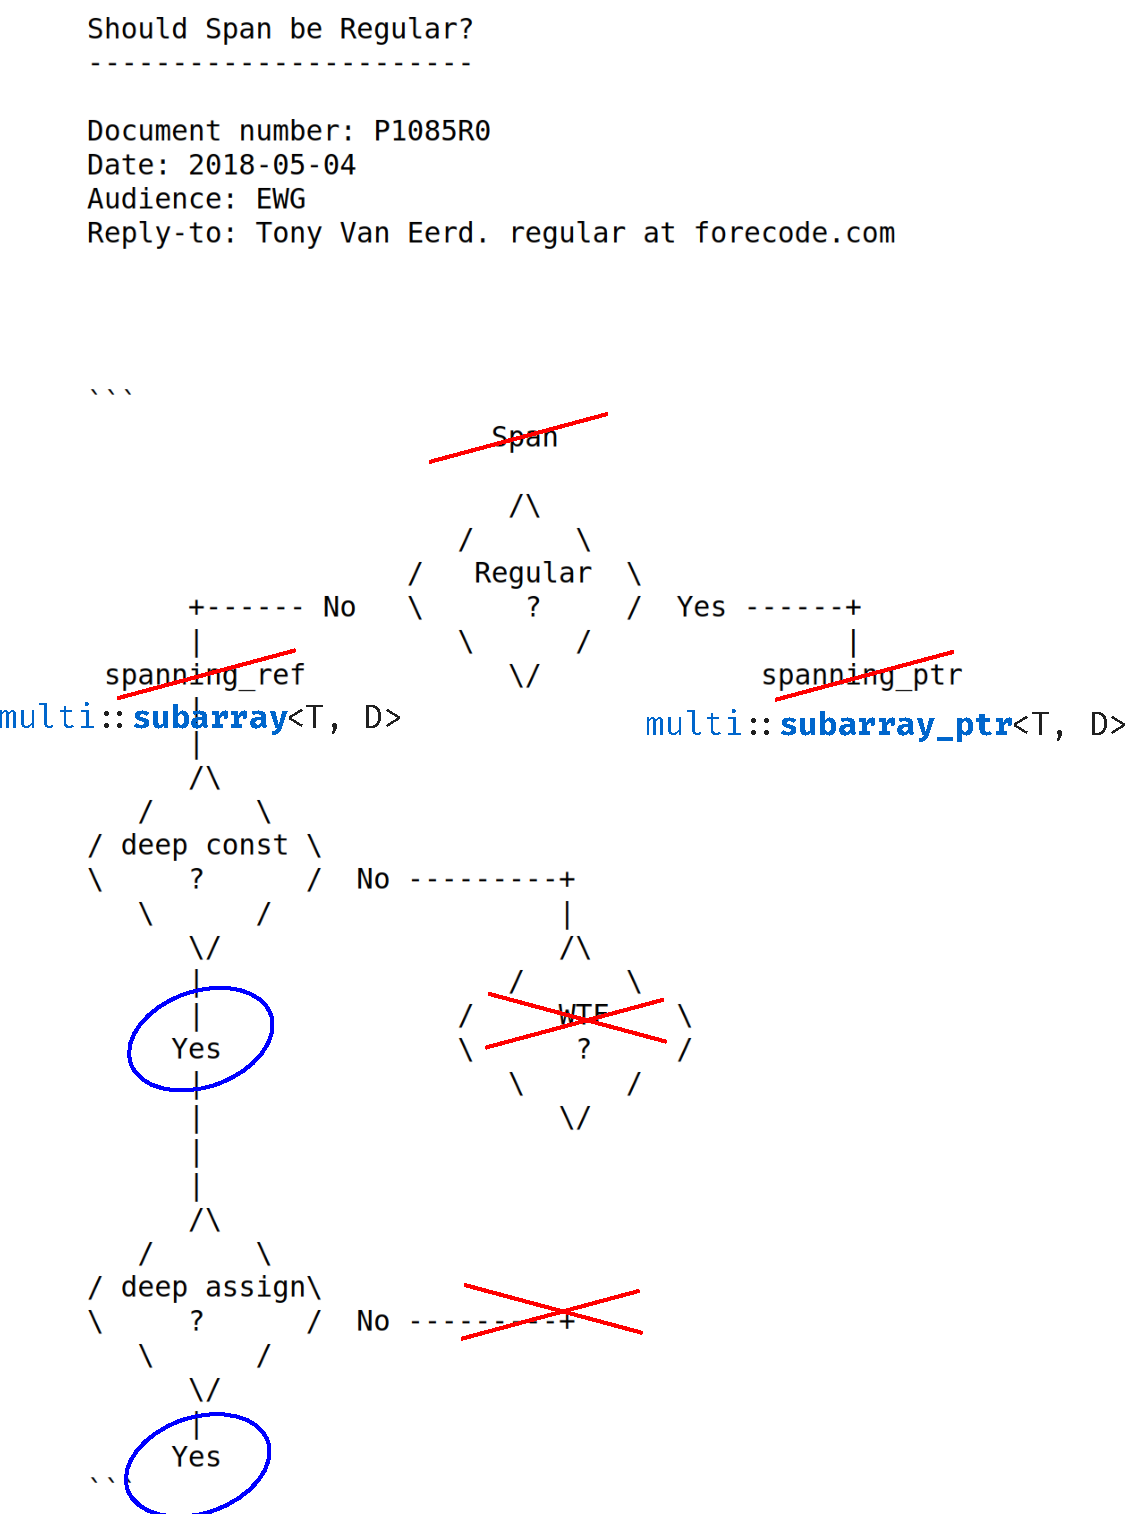
\includegraphics[trim=0 600 0 0, clip, scale=0.5]{nospan}
\end{column}
\begin{column}{0.5\textwidth}
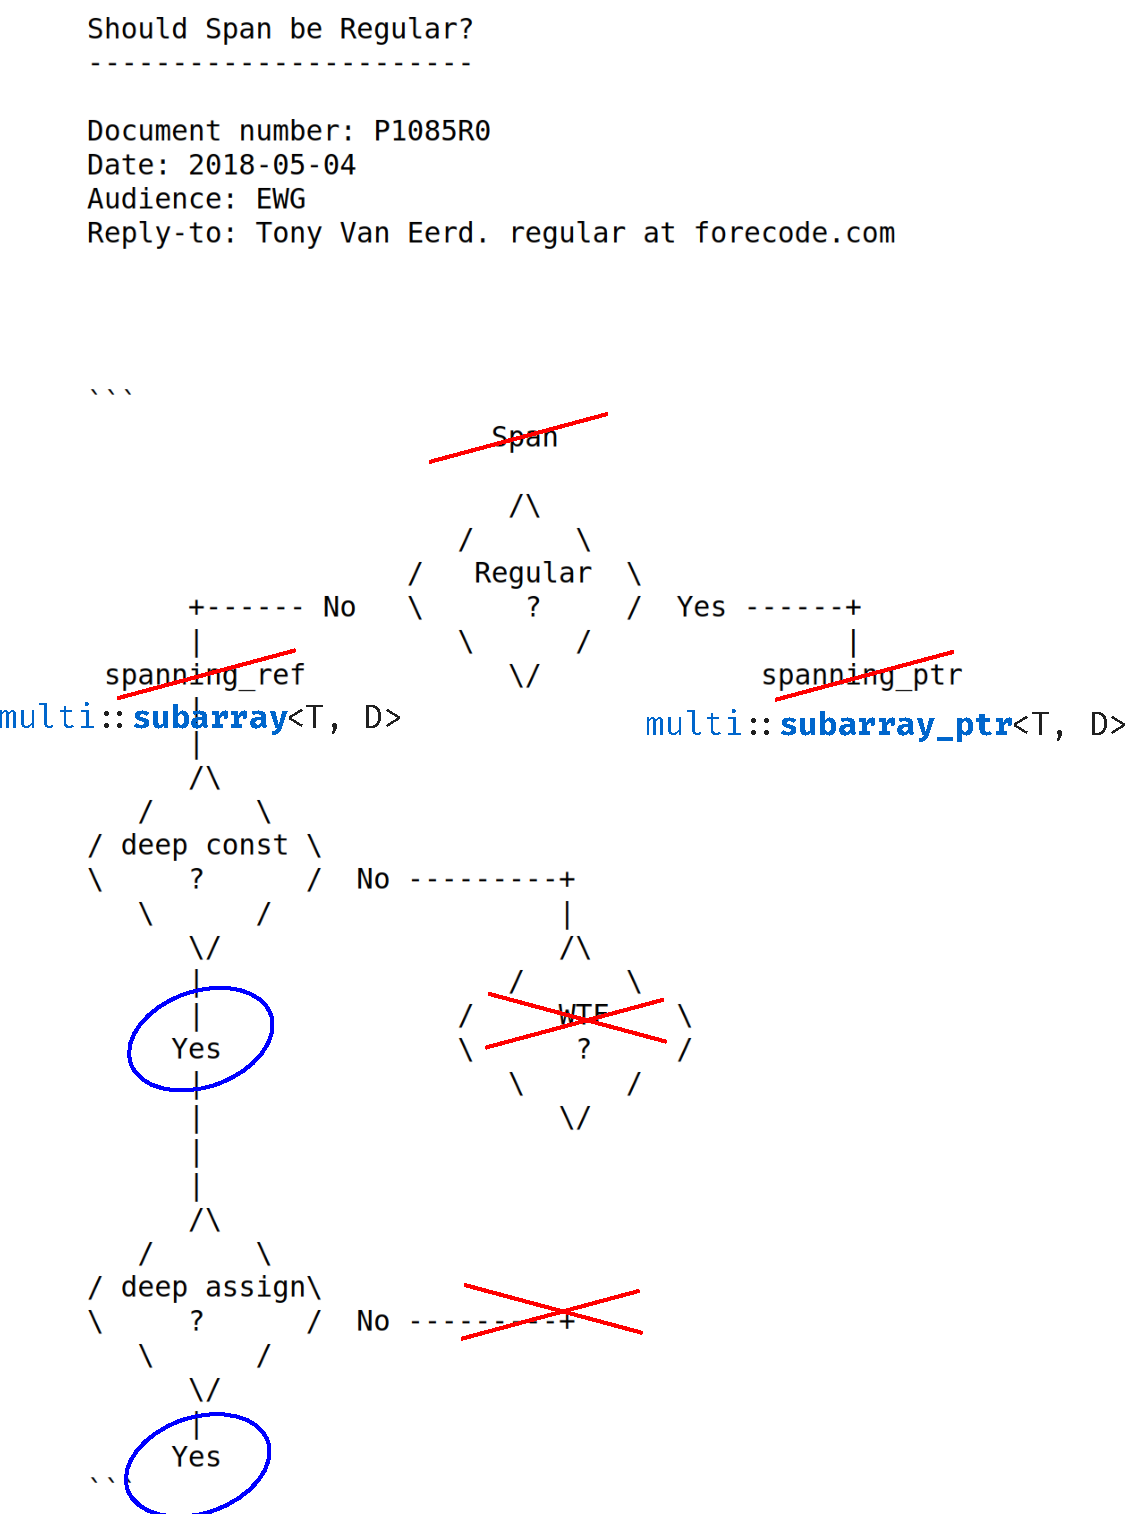
\includegraphics[trim=0 0 0 195, clip, scale=0.37]{nospan}
\end{column}
\end{columns}
\end{frame}

\begin{frame}[fragile]{\texttt{multi::dynamic\_array}: pinned owning array, \texttt{multi::inplace\_array}}

\lstinline|multi::dynamic_array<T, D, A>| owns memory, is copyable, but \textbf{not movable}:

\begin{lstlisting}
multi::dynamic_array<double, 2> D({3, 4});  // allocates, fixed size
multi::dynamic_array<double, 2> E = D;      // ok: deep copy
multi::dynamic_array<double, 2> F = std::move(D);  // ok, but O(N)
\end{lstlisting}

\begin{itemize}
  \item Size is fixed at construction (no \lstinline|resize|, no reallocation)
  \item Iterators and pointers are \textbf{never invalidated} after construction
  \item Iterators, subarrays, and pointers never invalidated unless the object is destroyed
\end{itemize}

\begin{block}{Inspired by \texttt{std::dynarray} (proposed for C++14, N3467, Stroustrup et al.)}
  \texttt{std::dynarray} was proposed as a fixed-size heap array
  but did not make it into the standard.
  \texttt{multi::dynamic\_array} generalizes the idea to $N$ dimensions.
\end{block}

\begin{lstlisting}
template<class T, dimensionality_type D, std::size_t Capacity = 32>
using inplace_array = multi::dynamic_array<T, D, multi::detail::static_allocator<T, Capacity>>;
\end{lstlisting}

\end{frame}

\begin{frame}[fragile]{Looks complicated, does it work? Test 1/2}
Regularity of \lstinline|multi::array<T, D>|:

The \textit{litmus} test for Regular types:
\begin{lstlisting}
std::vector<multi::array<int, 2>> V = { a1, a2, a3 };
std::sort( V.begin(), V.end() );
std::is_sorted( V.begin(), V.end() );
\end{lstlisting}
{\raggedleft\href{https://godbolt.org/z/df634c63G}{\texttt{godbolt.org/z/df634c63G}}\par}

{
\setbeamercolor{block title alerted}{fg=white, bg=green!60!black}
\setbeamercolor{block body alerted}{bg=green!10}
\begin{alertblock}{Passes!}
  Arrays have total order (if elements have total order),
  and behave like Regular
\end{alertblock}
}

\begin{alertblock}{The test is not about sorting... (not often used for arrays)}
  ... it is about showing that all the intermediate components work.
\end{alertblock}

\end{frame}

\begin{frame}[fragile]{Looks complicated, does it work? Test 2/2}

The \textit{acid} test (``[...] STL algorithms [...] exist to implement in-place stable sort'' -- Sean Parent, \emph{No Raw Loops} (2023))

\begin{lstlisting}
multi::array<int, 2> A = {{ 8, 6,  7},
                          {30, 1,  2},
                          { 8, 9, 11}};
std::sort( A.begin(), A.end() );
std::is_sorted( A.begin(), A.end() );
// {{ 8, 6,  7},
//  { 8, 9, 11},
//  {30, 1,  2}}
\end{lstlisting}
{\raggedleft\href{https://godbolt.org/z/eGK1T5j4M}{\texttt{godbolt.org/z/eGK1T5j4M}}\par}

{
\setbeamercolor{block title alerted}{fg=white, bg=green!60!black}
\setbeamercolor{block body alerted}{bg=green!10}
\begin{alertblock}{Passes!}
  Indicates that our iterators work correctly with \lstinline|swap|, \lstinline|std::rotate|, \lstinline|stable_partition|
\end{alertblock}
}

\begin{alertblock}{The litmus/acid tests are similar but prove different things}
  One test value semantics, the other test iterator infrastructure
\end{alertblock}

\begin{alertblock}{Again, the test is not about sorting...}
  ... it is about components.
\end{alertblock}

\end{frame}

\begin{frame}[fragile]{Looks complicated, does it work? Bonus Test}
\begin{lstlisting}
multi::array<int, 2> A = {{ 8, 6,  7},
                          {30, 1,  2},
                          { 8, 9, 11}};
std::sort( A.transposed().begin(), A.transposed().end() );
assert( std::is_sorted( A.transposed().begin(), A.transposed().end() ) );
// {{6,  7,  8},
//  {1,  2, 30},
//  {9, 11,  8}}
\end{lstlisting}
{\raggedleft\href{https://godbolt.org/z/1zdEfnPK9}{\texttt{godbolt.org/z/1zdEfnPK9}}\par}

{
\setbeamercolor{block title alerted}{fg=white, bg=green!60!black}
\setbeamercolor{block body alerted}{bg=green!10}
\begin{alertblock}{Passes!}
  Indicates that our iterators work correctly with \lstinline|swap|, \lstinline|std::rotate|, \lstinline|stable_partition|
\end{alertblock}
}

\begin{block}{}
  Also works with std::ranges algorithms, filters, etc.
\end{block}
\end{frame}

\begin{frame}[fragile]{Generic Serialization (\textbf{Boost.Serialization} and \textbf{Cereal})}

\begin{columns}[T]
\begin{column}{0.5\textwidth}
\begin{lstlisting}
#include <boost/archive/xml_oarchive.hpp>

multi::array<int, 2> A({10, 10});
std::ofstream ofs{"data.xml"};
boost::archive::xml_oarchive xoa{ofs};
xoa << boost::make_nvp("A", A);
\end{lstlisting}
\end{column}
\begin{column}{0.5\textwidth}
\begin{lstlisting}
#include <boost/archive/xml_iarchive.hpp>

multi::array<int, 2> B;
std::ifstream ifs{"data.xml"};
boost::archive::xml_iarchive xia{ifs};
xia >> B;
\end{lstlisting}
\end{column}
\end{columns}

\begin{center}
  \includesvg{serialization}
\end{center}
\end{frame}

\begin{frame}[fragile,label=allocator1]{Allocator support (The allocator controls where memory lives)}

\lstinline|multi::array<T, D, Allocator>| --- the allocator controls where memory lives:

Standard:
\begin{itemize}
  \item Classic (stateless allocators)
  \item Scoped allocators (propagated nested allocators)
  \item Polymorphic allocators \lstinline|std::pmr::polymorphic_allocator -> multi::pmr::array<T,D>|
\end{itemize}

Fancy:
\begin{itemize}
  \item Interprocess Allocator (memory mapped) \lstinline|boost::interprocess::allocator|
\end{itemize}

Special purpose:
\begin{itemize}
  \item \lstinline|thrust::device_allocator -> multi::thrust::device_array<T,D>| (device memory)
  \item \lstinline|thrust::universal_allocator -> multi::thrust::universal_array<T,D>| (unified memory)
  \item \lstinline|thrust::mr::allocator| (with custom memory resources)
\end{itemize}
\end{frame}

\begin{frame}[fragile,label=allocator2]{Allocator $\Rightarrow$ pointer type $\Rightarrow$ memory location}

\lstinline|std::allocator_traits<A>::pointer| is not always \lstinline|T*|:

\medskip
\begin{tabular}{@{}lll@{}}
\hline
\textbf{Allocator} & \textbf{Pointer type} & \textbf{Memory} \\
\hline
\lstinline|std::allocator<T>|                        & \lstinline|T*|                                 & CPU \\
\lstinline|std::pmr::polymorphic_allocator<T>|       & \lstinline|T*|                                 & PMR \\
\lstinline|thrust::device_allocator<T>|              & \lstinline|thrust::device_ptr<T>|              & GPU \\
\lstinline|thrust::universal_allocator<T>|           & \lstinline|thrust::universal_ptr<T>|           & CPU+GPU \\
\lstinline|thrust::omp::allocator<T>|                & \lstinline|thrust::omp::pointer<T>|            & OpenMP \\
\lstinline|boost::interprocess::allocator<T,...>|    & \lstinline|boost::interprocess::offset_ptr<T>| & Shared memory \\
\hline
\end{tabular}

\medskip

\begin{alertblock}[label=allocator3]{From WHERE to HOW}
The library propagates the pointer type throughout subarrays, iterators,
and references; all carry the allocator's pointer.
There is compile-time information on HOW to run.
\end{alertblock}

Both the library and the user can exploit this information.

\end{frame}

\begin{frame}[t,fragile,label=allocator4]{Algorithm Dispatching inside the library}
\begin{columns}[T]
\begin{column}{0.4\textwidth}
\begin{lstlisting}

multi::array<int, 2> A({10, 10});
multi::array<int, 2> B({10, 10});

B = A;
\end{lstlisting}
\end{column}
\begin{column}{0.6\textwidth}
\begin{lstlisting}
using alloc = thrust::device_allocator<int>;
multi::array<int, 2, alloc> A({10, 10});
multi::array<int, 2, alloc> B({10, 10});

B = A;
\end{lstlisting}
\end{column}
\end{columns}
\begin{lstlisting}
template<typename T, dimensionality_type D, class Alloc>
class array {
 using element_ptr = std::allocator_traits<Alloc>::pointer;
 auto operator=(array const& other) -> array& {
   adl_copy_n(other.elements().begin(), other.elements().end(), elements().begin());
\end{lstlisting}
\begin{center}
\includesvg{dispatching}
\end{center}
\end{frame}

\begin{frame}[fragile]{Algorithm Dispatching inside the library}
\begin{lstlisting}
class adl_copy_n_t {
  auto _(priority<0>, auto... as) ... {return std::copy_n(...);}    // CPU fallback
  auto _(priority<1>, auto... as) ... {return thrust::copy_n(...);} // GPU
  auto _(priority<2>, auto... as) ... {return copy_n(...);}         // ADL
  auto _(priority<3>, auto it, auto... rst) ... {return it.copy_n(...); } // member
public:
  template<class... As> auto operator()(As&&... as) const -> decltype(...) {
    return _(priority<3>(), std::forward<As>(as)...);
  }
};
inline constexpr adl_copy_n_t adl_copy_n;
\end{lstlisting}

\medskip
\begin{itemize}
  \item Overload resolution picks the \emph{highest priority} that compiles (SFINAE)
  \item Same call site works for CPU (\lstinline|std::|), GPU (\lstinline|thrust::|), or user types
  \item Extensible (intrusive): add members: add a \lstinline|copy_n| member function
\end{itemize}

\end{frame}

\begin{frame}[fragile,label=inq2]{\texttt{gpu::array}: Portable CPU/GPU Arrays via a Type Alias}
\begin{lstlisting}
// external_libs/gpurun/include/gpu/array.hpp:112
namespace gpu {
template<class type, size_t dim,
#ifdef ENABLE_GPU
    class allocator = caching_allocator<type>  // unified GPU memory
#else
    class allocator = std::allocator<type>     // ordinary CPU heap
#endif
>
using array = boost::multi::array<type, dim, allocator>; }
\end{lstlisting}
\vspace{0.5em}
\begin{itemize}
  \item \texttt{gpu::array<T,N>} \textbf{is} a \texttt{boost::multi::array<T,N,Alloc>}
  \item The allocator switches at compile time: GPU builds use
        \texttt{thrust::universal\_allocator} (visible to both CPU and GPU);
        CPU builds use \texttt{std::allocator}
  \item All multi indexing, slicing, and algorithm support is inherited unchanged
  \item No code change needed between CPU and GPU paths
\end{itemize}

\vspace{0.3em}
\tiny\texttt{external\_libs/gpurun/include/gpu/array.hpp:119}
\end{frame}

\begin{frame}[fragile,label=inq3]{Custom-Typed 1D Arrays for Atomic Properties}
\begin{lstlisting}
// Arrays of physical quantities -- element type can be anything
multi::array<vector3<double>, 1> forces(geo.size());
multi::array<double, 1>         charges(geo.size());

for(int ii = 0; ii < geo.size(); ii++)
    charges[ii] = atomic_pot
        .pseudo_for_element(geo.species(ii))
        .valence_charge();

interaction_energy(geo.size(), cell, charges,
                   geo.positions(), atomic_pot.range_separation(),
                   energy, forces);
\end{lstlisting}
\textit{Multi arrays are generic: \texttt{vector3<double>} is a valid element type,
giving a 1D array of 3-vectors representing per-atom forces.}

\vspace{0.3em}
\tiny\texttt{src/ionic/interaction.hpp:317}
\end{frame}

\begin{frame}[fragile,label=inq4]{Dynamic Resizing: k-points $\times$ Eigenstates}
\begin{lstlisting}
gpu::array<double, 2> eigenvalues_;
gpu::array<double, 2> occupations_;
...
// 2D arrays sized at runtime from MPI-distributed k-point data
eigenvalues_.reextent({n_kpin, max_local_spinor_set_size_});
occupations_.reextent({n_kpin, max_local_spinor_set_size_});
\end{lstlisting}
\vspace{0.5em}
\begin{itemize}
  \item \texttt{reextent} resizes without invalidating the element type
  \item Dimensions come from the MPI partition of k-points and states
  \item The same syntax works for CPU and GPU arrays (\texttt{gpu::array})
\end{itemize}

\vspace{0.3em}
\tiny\texttt{src/systems/electrons.hpp:188}
\end{frame}

\section{Lazy Arrays \& Restrictions}

\begin{frame}[fragile]{Lazy sequences, the evolution of iota}

Standard:
  \begin{lstlisting}
std::iota(c.begin(), c.end(), 0);  // c = {0, 1, 2, 3, ...}
  \end{lstlisting}
  \begin{lstlisting}
std::views::iota(1, 10);  // {1, ..., 9}
  \end{lstlisting}

In the library:
  \begin{lstlisting}
multi::array<char, 1> A = ...;
A            // {'a', 'b', 'c', 'd'}
A.extent();  // {  0,   1,   2,   3}
A.size();    //   4
  \end{lstlisting}
  \begin{lstlisting}
multi::array<int, 2> B = ...;
B.extent();  // leading dimension {0, 1, 2, 3, ..., B.size() - 1}
  \end{lstlisting}

\end{frame}

\begin{frame}[fragile]{Lazy array, multidimensional iota}

  \begin{lstlisting}[escapechar=|]
multi::array<char, 2> B = ...;
B.extent|\xout{s}|();  // leading dimension {0, 1, 2, 3, ..., B.size() - 1}
  \end{lstlisting}

  \begin{lstlisting}[escapechar=|]
multi::array<char, 2> B = {
  {'a', 'b', 'c'},
  {'d', 'e', 'f'}
};
B.extent|\uline{s}|();  // structured Cartesian product
% {
%   { tuple{0, 0}, tuple{0, 1}, tuple{0, 2} },  % <-- B.extents().begin()
%   { tuple{1, 0}, tuple{1, 1}, tuple{1, 2} }
% }

B.extent|\uline{s}|().elements();  % {tuple{0, 0}, tuple{0, 1}, tuple{0, 2}, tuple{1, 0},...}
B.extent|\uline{s}|().elements().begin() -- ... -- .end()

% std::views::cartesian_product( get<0>(B.extents()), get<1>(B.extents()) );
\end{lstlisting}

\end{frame}

\begin{frame}[fragile]{Initialize from coordinates function}
    \begin{center}
    \tornpaper{
        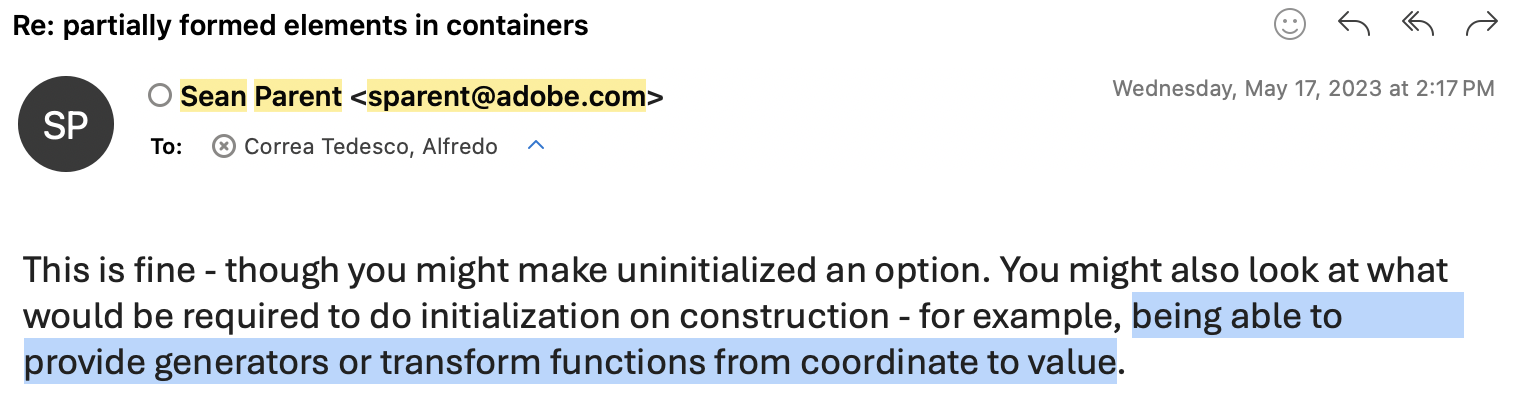
\includegraphics[height=0.4\textheight]{parent_coordinates}
    }
    \end{center}
\pause
    \begin{itemize}
    \item[\emoji{thinking-face}] \lstinline|multi::array<int, 2> A({10, 10}); set_from_coordinates(A, [](auto i, auto j) { return i + j; });| ???
    \item[\emoji{thinking-face}] \lstinline|multi::array<int, 2> const A({10, 10}, [](auto i, auto j) { return i + j; });| ???
    \item[\emoji{light-bulb}]    \lstinline|multi::array<int, 2> const A( ...special range with coordinates... ); A = ...|
    \end{itemize}
\end{frame}

\begin{frame}[fragile]{Restriction (mathematics)}{from Wikipedia}
\begin{quote}
  [...] In mathematics, the restriction of a function \(f\)
  is a new function, denoted \(f |_A\) or \(f \upharpoonright A\),
  obtained by choosing a smaller domain \(A\)
  for the original function \(f\).
  The function \(f\) is then said to extend \(f \upharpoonright A\). [...]
\end{quote}


Translated to C++, \(f\) could be a function object that maps coordinates to values, and
\(A\) can be a Cartesian set of points (of the array)

\pause

\begin{lstlisting}
multi::???({2, 3}, [](auto i, auto j) { return i + j; });

[](auto i, auto j) { return i + j; } ^ multi::extents_t{2, 3};

% {
%   { f(0, 0), f(0, 1), f(0, 2) },  % <-- .begin()
%   { f(1, 0), f(1, 1), f(1, 2) }
% }
\end{lstlisting}

\end{frame}

\begin{frame}[fragile]{General lazy arrays: function restricted to a domain}

A \lstinline|multi::restriction|
is the restriction (in the mathematical sense) of a function to a bounded index domain.

\begin{lstlisting}
% lazy 2x3 array R[i][j] = i + j, no memory allocated
auto R = multi::restriction({2, 3}, [](auto i, auto j) { return i + j; });

% equivalent idiomatic form using the ^ operator ("restricted to")
auto R = [](auto i, auto j) { return i + j; } ^ multi::extensions_t{2, 3};

R[1][2];           % 3         (computed on access)
R.size();          % 2
R.num_elements();  % 6
+R;                % materialize into multi::array<int, 2>
\end{lstlisting}

\medskip
Models the Multi array concept --- it has \lstinline|extents|, iterators, \lstinline|operator[]|, etc.\\
Structural operations compose (still) without allocating: \lstinline|transposed|, \lstinline|repeated|, \lstinline|diagonal|, \lstinline|partitioned|, \lstinline|reversed|, \lstinline|rotated|, \lstinline|transformed|, \lstinline|element_transformed|.
\end{frame}

\section{Algorithms \& Performance}

\begin{frame}[label=alg0]{Algorithms (raw loops)}
Take a 64x64x64 array (\(\sim 250\mathrm{k}\) elements) \lstinline|A|, apply a compute-bound op.

\begin{center}
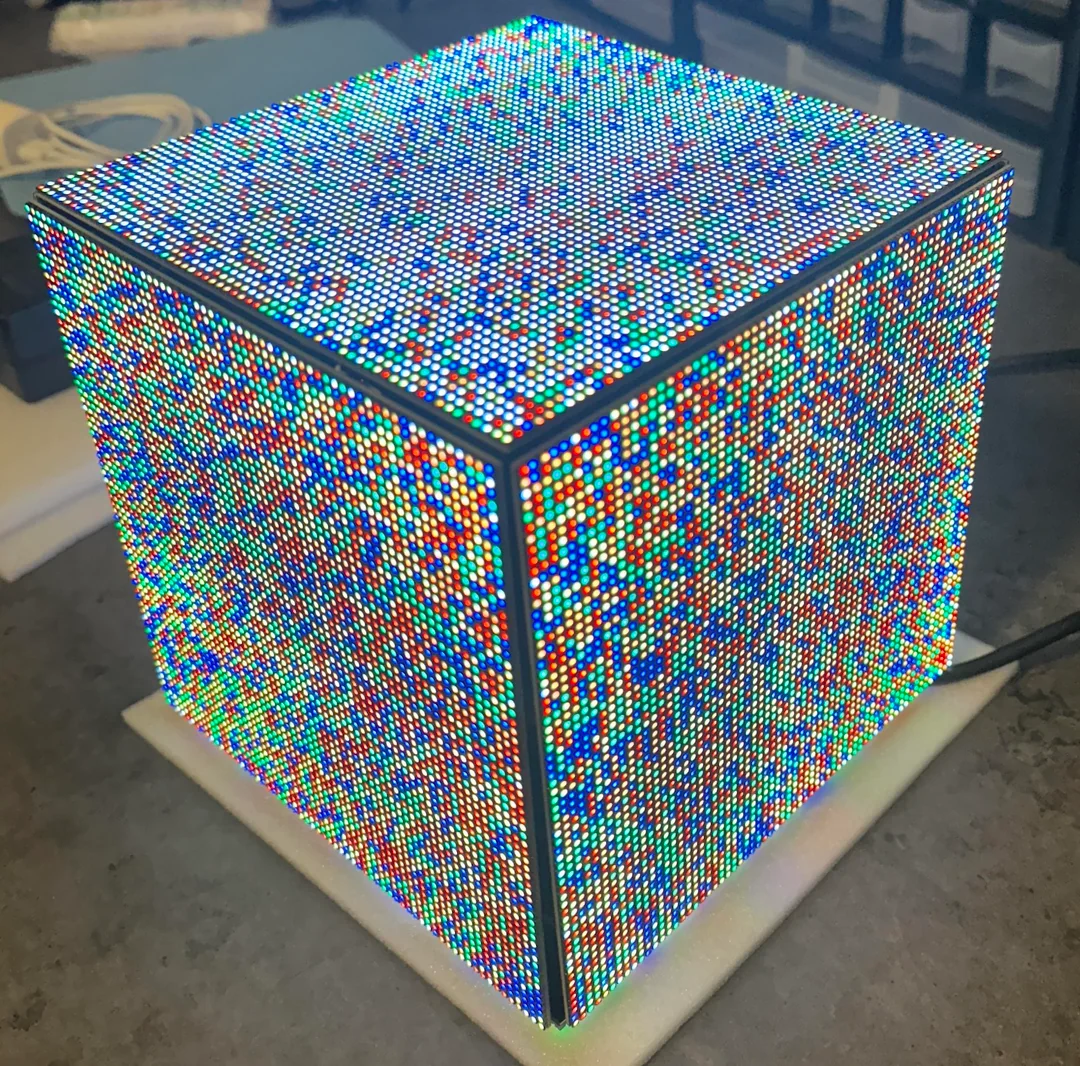
\includegraphics[width=0.4\textwidth]{led-cube.png}
\end{center}

\end{frame}

\begin{frame}[fragile,label=algo1]{Algorithms (raw loops)}
  Take a 64x64x64 array ($\sim 250$k elements) \lstinline|A|, apply a compute-bound op.

\begin{columns}[t]
\begin{column}{0.48\textwidth}
\textit{Index-based (coordinate access)}
\begin{lstlisting}
auto [is, js, ks] = A.extents();
for(auto i : is)
  for(auto j : js)
    for(auto k : ks)
      A[i][j][k] = op(A[i][j][k]);
\end{lstlisting}
\end{column}
\begin{column}{0.48\textwidth}
\textit{Range-for (element access)}
\begin{lstlisting}

for(auto&& plane : A)
  for(auto&& row : plane)
    for(auto&& elem : row)
      elem = op(elem);
\end{lstlisting}
\end{column}
\end{columns}

  timing: \textbf{2.6 msec}
\end{frame}

\begin{frame}[fragile,label=algo2]{Algorithms (algorithm seasoning)}
  Take a 64x64x64 array (\(\sim 250\mathrm{k}\) elements) \lstinline|A|, apply a compute-bound op.
  \begin{lstlisting}
std::for_each(     A.begin(), A.end(),
  [](auto&& plane) {
    for(auto&& row : plane) {
      for(auto&& elem : row) {
        elem = op(elem);
      }
    }
  }
);
  \end{lstlisting}
  timing: \textbf{2.6 msec}
\end{frame}

\begin{frame}[fragile,label=algo3]{Algorithms (algorithm parallelization)}
  Take a 64x64x64 array (\(\sim 250\mathrm{k}\) elements) \lstinline|A|, apply a compute-bound op.
  \begin{lstlisting}
std::for_each(std::execution::par, A.begin(), A.end(),
  [](auto&& plane) {
    for(auto&& row : plane) {
      for(auto&& elem : row) {
        elem = op(elem);
      }
    }
  }
);
  \end{lstlisting}
  timing: \textbf{1.4 msec}
\end{frame}

\begin{frame}[fragile,label=algo4]{Algorithms (attempt to parallelize in the GPU)}
  Take a 64x64x64 array (\(\sim 250\mathrm{k}\) elements) \lstinline|A|, apply a compute-bound op.
  \begin{lstlisting}
thrust::for_each(thrust::cuda::par, A.begin(), A.end(),
  [](auto&& plane) __device__ {
    for(auto&& row : plane) {
      for(auto&& elem : row) {
        elem = op(elem);
      }
    }
  }
);
  \end{lstlisting}
  timing: \pause doesn't compile! (Thrust is unfriendly to proxy objects)

  But even if it did compile... 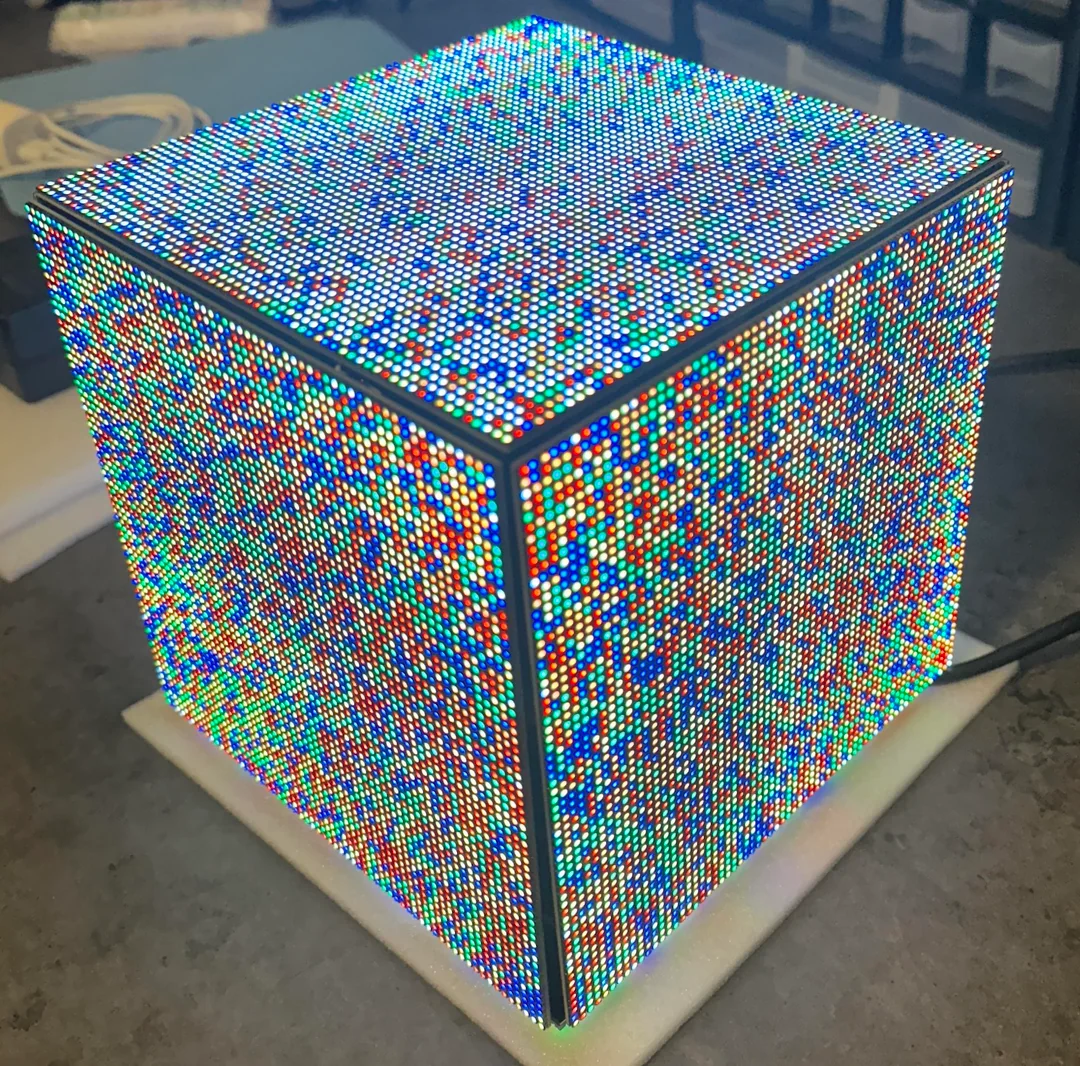
\includegraphics[width=0.12\textwidth]{led-cube.png}
\end{frame}

\begin{frame}[fragile,label=algo5]{Algorithms (optimized)}
  Take a 64x64x64 array (\(\sim 250\mathrm{k}\) elements) \lstinline|A|, apply a compute-bound op.
  \begin{lstlisting}
thrust::for_each(thrust::cuda::par, A.elements().begin(), A.elements().end(), [] __device__(auto& e) {
  e = op(e);
});
  \end{lstlisting}
  timing: \textbf{0.3 msec}
\end{frame}

\begin{frame}[fragile,label=algo6]{Algorithms (optimized)}
  Take a 64x64x64 array (\(\sim 250\mathrm{k}\) elements) \lstinline|A|, apply a compute-bound op.
  \begin{lstlisting}
std::for_each(std::execution::par, A.elements().begin(), A.elements().end(), [] (auto& e) {
  e = op(e);
});
  \end{lstlisting}
  timing: \textbf{0.7 msec}
\end{frame}

\begin{frame}[fragile,label=algo7]{Summary of Algorithm optimization}

\begin{table}
\begin{tabular}{lcc}
\textbf{Algorithm} & \textbf{Time (ms)} & \textbf{Speedup} \\
\hline
Nested loops                                    & 2.6 & 1.0x \\
STL (leading dimension)                         & 2.6 & 1.0x \\
Parallel STL (leading dimension)                & 1.4 & 1.9x \\
\hline
thrust::for\_each ([cuda::par, ] flat elements) & 0.3 & 8.7x \\
std::for\_each (std::par, flat elements)        & 0.7 & 3.7x \\
std::for\_each (flat elements)                  & 3.0 & 0.9x \\
\end{tabular}
\end{table}

\begin{alertblock}{}
  Prefer algorithms to raw loops.
  Prefer to fuse loops.
\end{alertblock}

  \begin{lstlisting}
  algorithm(... A.elements() ...);
  \end{lstlisting}

\end{frame}

\begin{frame}[fragile,label=algo8]
\frametitle{...but I need my 3D structure}

Task: assign values based on the 3D indices

\begin{lstlisting}
auto [is, js, ks] = A.extents();
for(auto i : is) for(auto j : js) for(auto k : ks)
  A[i][j][k] = fun(i + j + k);
\end{lstlisting}

\begin{overprint}
\onslide<1| handout:0>
\begin{lstlisting}
std::for_each(
  A.extents().elements().begin(), A.extents().elements().end(),
  [&A](auto ijk) { auto [i, j, k] = ijk;
    A[i][j][k] = fun(i + j + k);
  }
);
\end{lstlisting}

\onslide<2| handout:1>
\begin{lstlisting}
std::transform(
  A.extents().elements().begin(), A.extents().elements().end(),
  A.elements().begin(),
  [](auto ijk) { auto [i, j, k] = ijk;
    return fun(i + j + k);
  }
);
\end{lstlisting}

Note: \lstinline|A.extents().elements().size() == A.elements().size()|
\end{overprint}

\end{frame}

\begin{frame}[fragile,label=gpurun1]{\texttt{gpu::run} --- portable loops \& reductions}

  Write the body \alert{once} as a lambda over indices; the same source
  compiles to a \textbf{CUDA/HIP kernel} (GPU) or a \textbf{\texttt{for} loop}
  (CPU), chosen by \texttt{ENABLE\_GPU}. \texttt{gpu::run} handles the launch
  config, bounds, and sync. \texttt{GPU\_LAMBDA} $=$ \texttt{\_\_device\_\_}
  on GPU, nothing on CPU; capture iterators by value.

  \begin{lstlisting}
// loop:   v[i] = i           (1D; also 2D/3D/4D overloads)
gpu::run(n, m, [v=begin(v)] GPU_LAMBDA (auto i, auto j){ v[i][j] = i + j; });

// scalar reduction:   sum_i a[i]
double s = gpu::run(gpu::reduce(n), 0.0,
                    [a=begin(a)] GPU_LAMBDA (auto i){ return a[i]; });

// vector reduction:   r[i] = sum_j m[i][j]
auto r = gpu::run(n, gpu::reduce(m), 0.0,
                  [M=begin(M)] GPU_LAMBDA (auto i, auto j){ return M[i][j]; });
  \end{lstlisting}
  \footnotesize
  \begin{itemize}
    \item \textbf{Loops:} \texttt{run(sizes..., kernel)} --- 1 to 4 index dimensions.
    \item \textbf{Reduce:} tag a dimension \texttt{gpu::reduce(\,)} to sum over it
          (GPU: \texttt{thrust} / shared-memory tree; CPU: nested loops).
    \item Free leading dimension $\Rightarrow$ vector result \texttt{gpu::array<T,1>};
          all reduced $\Rightarrow$ scalar.
  \end{itemize}
\end{frame}

\begin{frame}{Recipe to `port' your array code}
\begin{center}
  Convert your loops into algorithms (discover)\\
        \emoji{down-arrow}\\
      Flatten your algorithms (\lstinline|.elements()|, \lstinline|.extensions()|, lazy arrays)\\
        \emoji{down-arrow}\\
      Parallelize your algorithm (std::execution::par)\\
          \emoji{down-arrow}\\
      Change your memory space (use custom libraries if necessary, e.g. Thrust)
\end{center}
\end{frame}

\begin{frame}[fragile]{The Problem: Row-wise Reduction}

Given a 2D array, reduce each row:
\begin{lstlisting}
auto M    = multi::array<double, 2, thrust::device_allocator<double> >({100, 1000});
auto sums = multi::array<double, 1, thrust::device_allocator<double> >(M.size(0));

thrust::transform(M.begin(), M.end(), sums.begin(),
  [](auto const& row) {
    return thrust::reduce(row.begin(), row.end());
  }
);
\end{lstlisting}
\centering
\includesvg[scale=1.2]{reduce_by_row}

\textbf{Problem:} Missed opportunity for parallelization
\end{frame}

\begin{frame}[fragile]{Solution: use Thrust's \texttt{reduce\_by\_key}}
\centering
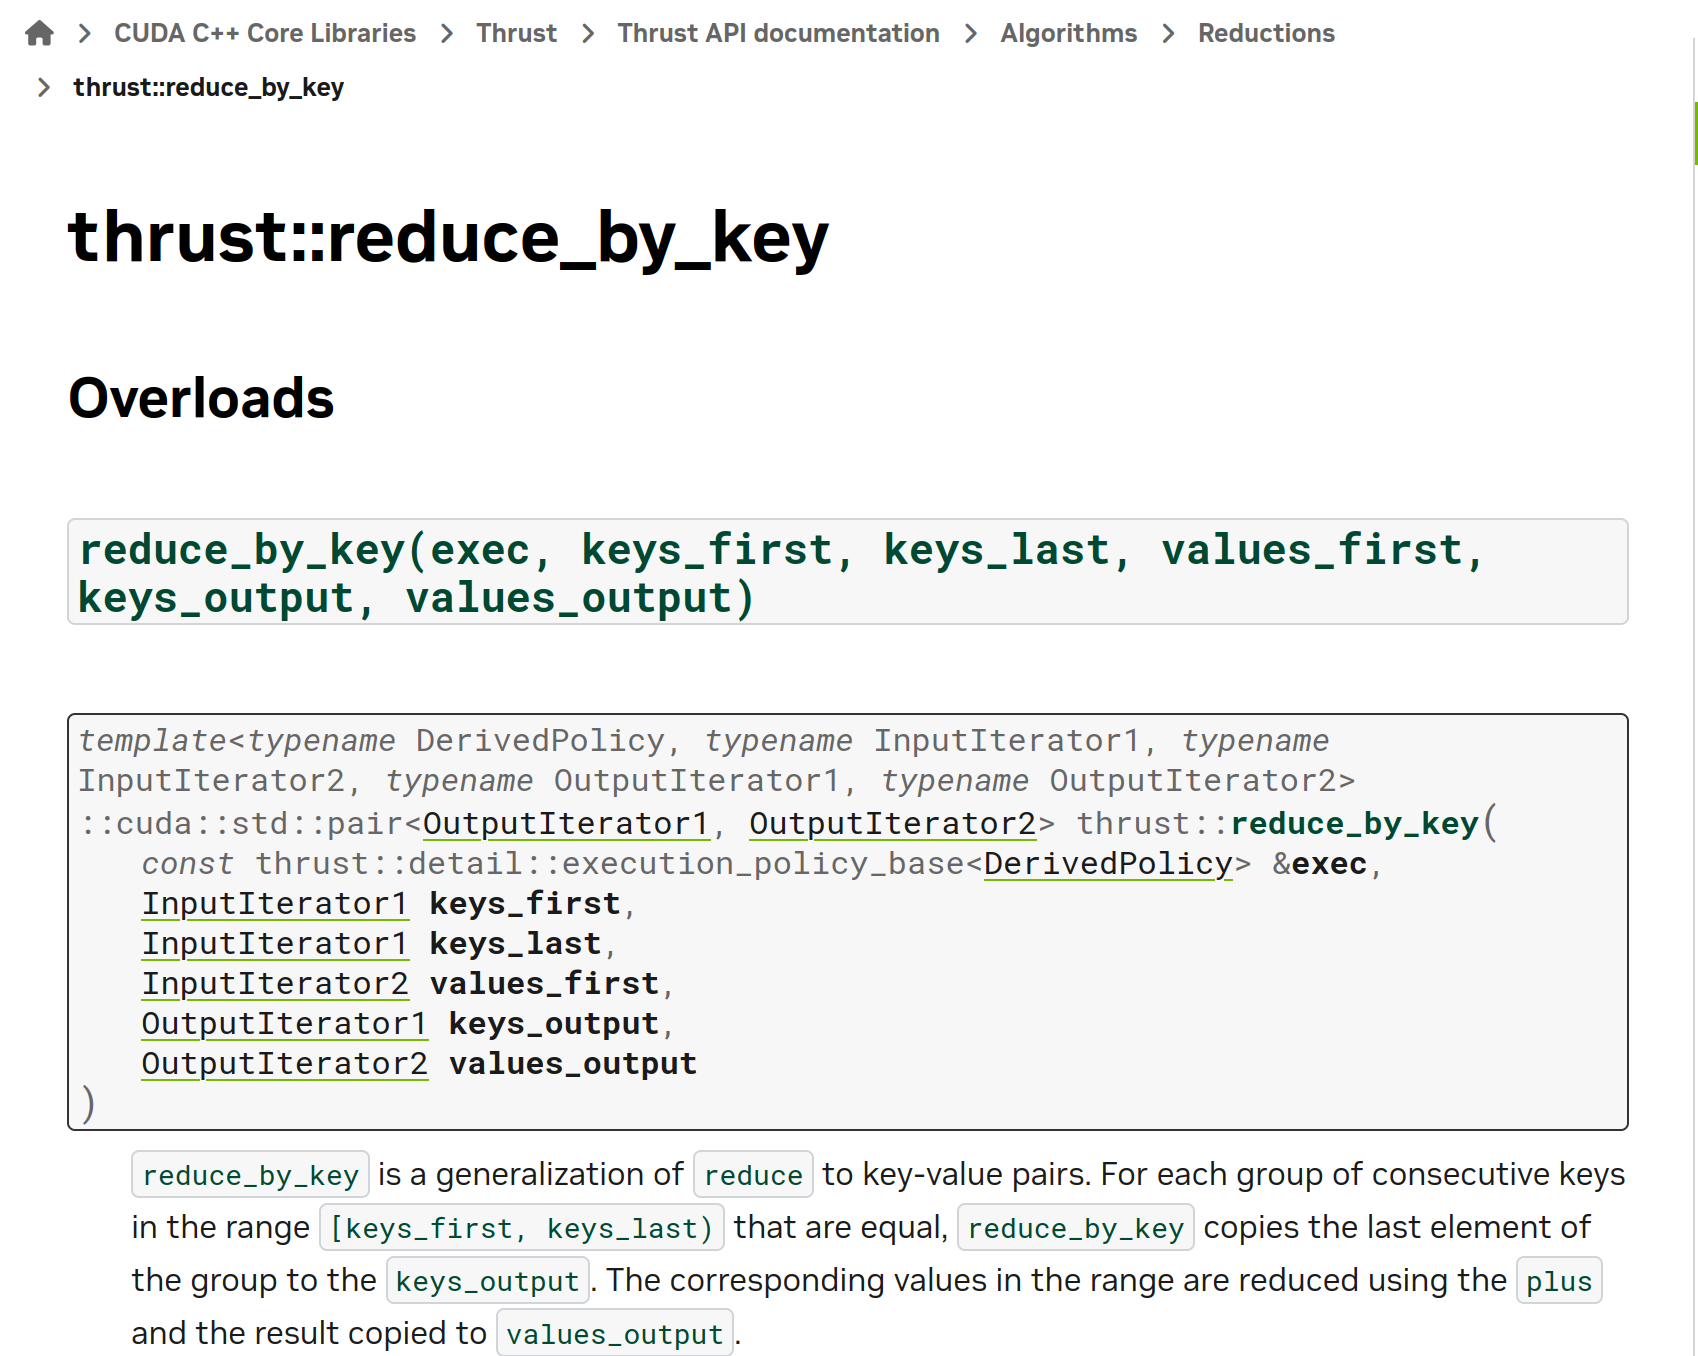
\includegraphics[scale=0.15]{reduce_by_key_doc}
~\includesvg[scale=1.4]{reduce_by_key}
\end{frame}

\begin{frame}[fragile]{Solution: Implement \texttt{reduce\_by\_row} }

\begin{lstlisting}
template<class ExecutionPolicy, class T, class S>
auto reduce_by_row(ExecutionPolicy&& ep, T const& M, S&& sums) -> S&& {
  assert(M.extension() == sums.extension());
  auto row_idx = []__host__ __device__ (int i, int j){return i;} ^ M.extensions();

  ::thrust::reduce_by_key(
    ep,
    row_idx.elements().begin(), row_idx.elements().end(),
    M.elements().begin(),
    ::thrust::make_discard_iterator(),
    sums.begin()
  );

  return std::forward<S>(sums);
}
\end{lstlisting}
All \(N_x \times N_y\) elements processed in parallel; no serial loop over rows.
\end{frame}

\begin{frame}[fragile]{reduce\_by\_index: lazy arrays}

Works directly on \lstinline|restriction|s --- no intermediate storage:
\begin{lstlisting}
multi::array<double, 1, thrust::device_allocator<double> > sums(nx);

reduce_by_row(
    [](multi::index ix, multi::index iy) { return ix * iy; }
    ^ multi::extensions_t<2>(nx, ny),   % lazy 2D array
    sums
);
\end{lstlisting}

\begin{itemize}
  \item No \lstinline|multi::array<double, 2>| ever allocated
  \item Values generated on-the-fly by each GPU thread
  \item Combines lazy evaluation with massively parallel reduction
\end{itemize}
\end{frame}

\begin{frame}{Recipe to `port' your array code (revisited)}
\begin{center}
  Convert your loops into algorithms (discover)\\
        \emoji{down-arrow}\\
      Flatten your algorithms (\lstinline|.elements()|, \lstinline|.extensions()|, lazy arrays)\\
        \emoji{down-arrow}\\
      Parallelize your algorithm (std::execution::par)\\
          \emoji{down-arrow}\\
      Change your memory space (use custom libraries if necessary, e.g. Thrust)\\
          \emoji{down-arrow}\\
      Keep looking for algorithms
  \end{center}
\end{frame}

\section{Adaptors \& Ecosystem}

\begin{frame}[label=adaptors1]{Adaptors}

Boost.Multi ships optional adaptors that integrate arrays with external libraries:

\begin{table}
\small
\begin{tabular}{lll}
\textbf{Header} & \textbf{Library} & \textbf{Purpose} \\
\hline
\lstinline|adaptors/blas.hpp|    & BLAS (cuBLAS, rocBLAS) & matrix/vector algebra \\
\lstinline|adaptors/lapack.hpp|  & LAPACK               & linear algebra (SVD, etc.) \\
\lstinline|adaptors/fftw.hpp|    & FFTW3                & FFT on CPU \\
\lstinline|adaptors/cufft.hpp|   & cuFFT                & FFT on NVIDIA GPU \\
\lstinline|adaptors/thrust.hpp|  & Thrust               & GPU/OMP parallel algorithms \\
\lstinline|adaptors/tblis.hpp|   & TBLIS                & tensor contractions \\
\lstinline|adaptors/mpi.hpp|     & MPI                  & distributed arrays \\
\end{tabular}
\end{table}

\begin{block}{}
  Adaptors are header-only and opt-in. Include only what you use.
\end{block}

\end{frame}

\begin{frame}[fragile,label=adaptors2]{Philosophy behind adaptors (BLAS/CUDA BLAS example)}

\begin{itemize}
  \item When possible, the same code should work for different backends
  \item Uses functional style of programming (deviates from \texttt{std::linalg})
  \item Efficient (no surprises)
\end{itemize}

\begin{columns}[T]
\begin{column}{0.45\textwidth}
\begin{lstlisting}

multi::array<double, 2>
  A({3, 3}), B({3, 3}), C({3, 3});
\end{lstlisting}
\end{column}
\begin{column}{0.55\textwidth}
\begin{lstlisting}
multi::array<double, 2, thrust::device_allocator<int>>
  A({3, 3}), B({3, 3}), C({3, 3});
\end{lstlisting}
\end{column}
\end{columns}
\begin{lstlisting}
C = blas::gemm(1.0, A, B);  // C = 1.0*A*B, shouldn't allocate
A = + blas::gemm(1.0, A, B);  // operator+ to break aliasing
\end{lstlisting}
\begin{center}
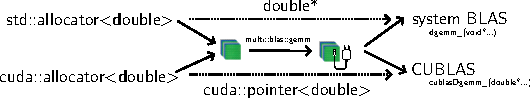
\includegraphics[scale=0.7]{dispatching_blas}
\end{center}

\lstinline{multi::blas::gemm} produces a "gemm" ranges;
custom \lstinline{copy_n} calls actual GEMM operation
\end{frame}

\begin{frame}[fragile,label=inq5]{4D Fields: Reinterpretation and Axis Rotation}
\begin{lstlisting}[language=C++]
// phi is a 4D array: [ix][iy][iz][istate]
// vector field stores complex3 elements; cast to scalar complex
// then rotate axes so [istate] becomes the leading dimension

auto&& fphi_as_scalar =
    fphi.hypercubic()
        .template reinterpret_array_cast<complex>(3)
        .rotated().rotated().rotated()  // bring [istate] to front
        .flatted()                      // merge spatial dims
        .rotated();                     // final layout for FFT

to_fourier_array(phi.basis(), fphi.basis(),
                 phi_as_scalar, fphi_as_scalar);
\end{lstlisting}
\textit{No data is copied: every operation returns a zero-cost view
with a different layout. The FFT routine sees a plain 2D array.}

\vspace{0.3em}
\tiny\texttt{src/operations/transform.hpp:206}
\end{frame}


\begin{frame}[fragile,label=inq6,shrink]{FFTW / cuFFT via a Unified Multi Adaptor}
\begin{lstlisting}
// operations/transform.hpp:23-25, 68-104

// {true,true,true,false}: transform dims 0,1,2 -- batch over dim 3 (states)
fft::dft_forward ({true, true, true, false}, array_rs, array_fs);
fft::dft_backward({true, true, true, false}, array_fs, array_rs);

// MPI-parallel: split into 1D + 2D passes with a transpose in between
fft::dft_forward({true, false, false, false}, array_rs, tmp);
parallel::transpose_forward(comm, ...);
fft::dft_forward({true, true,  false, false}, tmp, array_fs);

fft::dft_backward({true, true,  false, false}, array_fs, tmp);
parallel::transpose_backward(comm, ...);
fft::dft_backward({true, false, false, false}, tmp, array_rs);
\end{lstlisting}
\begin{itemize}
  \item The boolean mask selects \textit{which dimensions} to transform
  \item \texttt{fft::} and \texttt{fftw::} share the same interface ---
        only the \texttt{\#include} and namespace alias change
  \item MPI-distributed FFT is decomposed manually into 1D passes
        separated by an all-to-all transpose
\end{itemize}
\tiny\texttt{src/operations/transform.hpp:68}
\end{frame}

\begin{frame}[label=blasops]{Multi BLAS Adaptor: Operation Summary (selected examples)}
\footnotesize
\setlength{\tabcolsep}{5pt}
\begin{tabular}{@{}lll@{}}
\hline
\textbf{Operation} & \textbf{Out-parameter form} & \textbf{Functional form} \\
\hline
\multicolumn{3}{l}{\textit{Level 1 --- scalars from vectors}} \\[2pt]
\texttt{nrm2} $\|x\|_2$  & \texttt{blas::nrm2(x, r)}        & \texttt{double r = blas::nrm2(x)} \\
\texttt{asum} $\|x\|_1$  & \texttt{blas::asum(x, r)}        & \texttt{double r = blas::asum(x)} \\
\texttt{dot}  $x \cdot y$ & \texttt{blas::dot(x, y, r)}     & \texttt{double r = blas::dot(x, y)} \\[4pt]
\multicolumn{3}{l}{\textit{Level 1 --- vector updates}} \\[2pt]
\texttt{axpy} $y \mathrel{+}= \alpha x$ & \texttt{blas::axpy(a, x, y)}    & \texttt{y += blas::axpy(a, x)} \\[4pt]
\multicolumn{3}{l}{\textit{Level 2 --- matrix-vector}} \\[2pt]
\texttt{gemv} $y = \alpha Ax + \beta y$          & \texttt{blas::gemv(a, A, x, b, y)} & \texttt{y = blas::gemv(a, A, x)} \\[4pt]
\multicolumn{3}{l}{\textit{Level 3 --- matrix-matrix}} \\[2pt]
\texttt{gemm} $C = \alpha AB$          & \texttt{blas::gemm(a, A, B, b, C)} & \texttt{C = blas::gemm(a, A, B)} \\
\texttt{herk} $C = \alpha A A^\dagger$ & \texttt{blas::herk(fill, a, A, b, C)} & \texttt{C = blas::herk(a, A)} \\
\hline
\end{tabular}

\medskip
{\footnotesize\textbf{View manipulators} (usable as arguments above):
\texttt{blas::H(A)} — conjugate-transpose \quad
\texttt{blas::T(A)} — transpose \quad
\texttt{blas::C(x)} — conjugate}
\end{frame}

\begin{frame}[fragile,label=inq6,shrink]{BLAS / cuBLAS via the Multi BLAS Adaptor}
\begin{lstlisting}
// operations/overlap.hpp:33-45
namespace blas = boost::multi::blas;

// Overlap matrix: S_ij = dV * sum_k conj(phi1[k][i]) * phi2[k][j]
//   blas::H()  -- conjugate transpose (Hermitian adjoint)
//   gemm()     -- dispatches to BLAS (CPU) or cuBLAS (GPU)

// serial case: single gemm into the result block
olap.block() = blas::gemm(basis.volume_element(),
                           blas::H(phi1_matrix),
                           phi2_matrix);

// parallel case: compute locally, then MPI-reduce by block
auto arr = +blas::gemm(basis.volume_element(),
                          blas::H(phi1_matrix),
                          phi2_matrix);
\end{lstlisting}
\begin{itemize}
  \item \texttt{blas::gemm} and \texttt{blas::H} work on any \texttt{multi} array,
        CPU or GPU --- no code change needed
  \item The \texttt{+} prefix forces immediate evaluation into an owning array
  \item The same adaptor also provides \texttt{blas::nrm2}, \texttt{blas::gemv},
        \texttt{blas::trsm}, \ldots
\end{itemize}
\tiny\texttt{src/operations/overlap.hpp:33}
\end{frame}

\begin{frame}[label=adaptors]{Multiparadigm}
\centering
\begin{tikzpicture}[
    mindmap,
    scale=0.45, transform shape,
    concept color = red!30,
    every node/.style = {concept},
    grow cyclic,
    clockwise from = 90,
    level 1/.append style = {
        level distance = 4.5cm,
        sibling angle = 120
    },
    level 2/.append style = {
        level distance = 3cm,
        sibling angle = 45}
]
\node {\textsc{Multi}}
    child [concept color = blue!30] {node {Index access}
        child [grow=135] {node {Traditional loops}}
        child [grow=45]  {node {gpu::run}}
    }
    child [concept color = green!30] {node {Iterators}
        child [grow=375] {node {Standard Template Library}}
        child [grow=330] {node {CUDA Thrust}}
        child [grow=285] {node {Boost}}
    }
    child [concept color = magenta!30] {node {Raw access (adaptors)}
            child [grow=300, concept color = magenta!50!black] {node {BLAS/LAPACK}}
            child [grow=255, concept color = magenta!60!black] {node {FFTW}}
            child [grow=210, concept color = magenta!70!black] {node {cuBLAS}}
            child [grow=165, concept color = magenta!70!black] {node {cuFFT}}
            child [grow=120, concept color = magenta!70!black] {node {MPI}}
    };
\end{tikzpicture}
\end{frame}

\begin{frame}{Thoughts about AI}
  \begin{itemize}
    \item No AI was used to develop the library
    \item After Boost Review (conditionally accepted), AI was used to proofread documentation
    \item The irony isn't lost on me: I'm probably documenting mainly for AI
    \item ... but I'd prefer AI that learns to code using Generic Programming
  \end{itemize}
\end{frame}

\begin{frame}{Takeaways}

\begin{enumerate}
  \item \textbf{Generic programming works for arrays. (If you make some concessions \emoji{hot-pepper})}\\
    The same code handles 1D\ldots ND, CPU and GPU, owned and borrowed memory.

  \item \textbf{Views are cheap, copies are explicit.} (no need for reference counting or pointer/shallow semantics)\\
    Slicing, transposing, striding --- all return lightweight views over the same data.

  \item \textbf{Compose/expand with the STL, don't replace it with frameworks}\\
    Standard algorithms, execution policies, and iterators work out of the box.

  \item \textbf{Allocator = backend}\\
    Swap the allocator to move between CPU, CUDA, OpenMP --- no code changes.
\end{enumerate}
\vfill
\begin{center}
  Documentation\\
  \Large\href{https://correaa.gitlab.io/boost-multi/}{\texttt{correaa.gitlab.io/boost-multi}}\\
  \Large\href{https://correaa.github.io/boost-multi/}{\texttt{correaa.github.io/boost-multi}}
\end{center}

\end{frame}

%% ---- standalone bootstrap: close the document opened at the top ------------
\ifdefined\framesStandalone
  \end{document}
\fi

\end{document}
